\documentclass[11pt]{article}

\usepackage[margin=1in]{geometry}
\usepackage{amsmath, amssymb, amsthm, bm}
\usepackage{graphicx}
\usepackage{booktabs}
\usepackage{hyperref}
\usepackage{microtype}
\usepackage{pgfplots}
\pgfplotsset{compat=1.18}
\usepackage{tikz}

% Colorblind-safe series colors (color encodes the contract; dash style encodes the scenario)
\definecolor{vizblue}{HTML}{2A78D6}   % straight debt
\definecolor{vizorange}{HTML}{EB6834} % GDP-linked / contingent clause
\definecolor{vizgreen}{HTML}{008300}  % disaster clause

\usepackage[style=authoryear,sortcites=true,sorting=nyt,maxcitenames=2,maxbibnames=10,uniquename=false,uniquelist=false,backend=bibtex]{biblatex}
\addbibresource{references.bib}

\hypersetup{colorlinks=true, linkcolor=blue, citecolor=blue, urlcolor=blue}

\newtheorem{lemma}{Lemma}
\newtheorem{proposition}{Proposition}
\newtheorem{remark}{Remark}

\title{\bf Climate-Contingent Sovereign Finance:\\\large Extending Fiscal Limits to Logistical Climate Risk Transmission to Global Assets}
%\author{James K Rice \thanks{PhD Candidate, University of Essex (UK)}}
\date{\today}

\begin{document}
\maketitle

\begin{abstract}
Sovereigns exposed to climate risk have begun to write state contingency directly into their debt contracts: Grenada's 2015 restructuring and Barbados's 2018--19 restructuring and 2022 issuance include clauses that suspend debt service after qualifying natural disasters. This paper asks what such instruments do to fiscal limits. Building on the structural fiscal-limit framework of \textcite{CollardEtAl2015}, as extended to climate damages by \textcite{Seghini2026}, it makes two contributions. First, it generalizes the maximum sustainable borrowing and maximum sustainable debt objects (MSB/MSD) to a portfolio of state-contingent liabilities, so that the fiscal limit depends not only on mean growth but on how contractual repayments load on left-tail states. Second, it extends the framework from chronic physical risk---the focus of the baseline model---to acute physical risk in the NGFS sense, by introducing a Barro-style disaster process whose intensity can rise with cumulative emissions. A Monte Carlo illustration quantifies both margins: at the baseline calibration, a GDP-linked repayment clause raises the one-period analogue of maximum sustainable borrowing by 10--12 percent relative to straight debt and cuts the default probability at the issuance optimum by roughly two-thirds; the advantage grows with the rollover need and with the thickness of the left tail, is invariant to surplus capacity, and is maximized at an interior level of contractual relief. A disaster-triggered clause delivers smaller gains that are limited by basis risk, and a temperature-linked coupon adds value only when the coupling between global emissions realizations and domestic disaster intensity is strong. A reduced-form logistics-amplification channel linking supply-chain disruption to sovereign premia, and a monetary block covering collateral policy and asset purchases, are developed analytically; their full numerical solution and empirical calibration are beyond the scope of this paper, and they are treated as extensions in the appendices.
\end{abstract}

\textbf{Keywords:} Climate-Contingent Sovereign Debt; Maximum Sustainable Debt (MSD); State Debt Instruments; Climate Risk Transmission; Sovereign Risk Premia.

\section{Introduction}
\label{sec:intro}

A small but growing group of sovereigns now issues debt whose repayment terms respond automatically to climate-related events. Grenada's 2015 restructuring introduced a hurricane clause that defers debt service after a qualifying storm; Barbados incorporated natural-disaster clauses in its 2018--19 domestic and external restructurings and added pandemic clauses in its 2022 issuance; and climate-resilient debt clauses (CRDCs) are now offered by official-sector lenders, including UK Export Finance and the Inter-American Development Bank \parencite{imf_barbados2022_crdc,icma2022_crdc_chairs_summary,ukgov2023_crdc,cpi2025_crdc_primer,pina2022_scgd_database,OECD2021CatClauses}. Euro-area sovereigns have not adopted such clauses to date; they enter the analysis instead through the monetary-policy interface, because the Eurosystem is introducing climate-related adjustments to its collateral framework \parencite{ecb2025_climate_factor_pr}. The instruments themselves are concrete. Under Barbados's 2022 clause, a verified natural disaster exceeding a parametric trigger allows the government to suspend principal and interest payments for up to two years, with the deferred amounts capitalized: repayment obligations are moved out of exactly the states in which output has collapsed and fiscal capacity is at its weakest.

This paper asks what such instruments do to \emph{fiscal limits}---the maximum debt a sovereign can sustain without default becoming unavoidable. The central mechanic can be stated in one sentence: once climate shocks thicken the left tail of the growth distribution, maximum sustainable borrowing (MSB) and maximum sustainable debt (MSD) depend not only on mean growth but on \emph{how contractual repayments load on left-tail states}. Figure~\ref{fig:intro_loading} illustrates. A straight bond demands the same repayment in every state, so the default region is the entire set of growth outcomes in which repayment capacity $\alpha g$ falls below the promised face value. A contingent clause steps repayment down precisely in low-growth states, shrinking the default region---in the configuration drawn, cutting the probability mass in the default set from 8.0\% to 1.6\%---at the cost of a lower payoff in states where the sovereign would have repaid anyway. Whether that trade raises or lowers the fiscal limit is a quantitative question, and it is the question this paper answers.

\begin{figure}[!t]
\centering
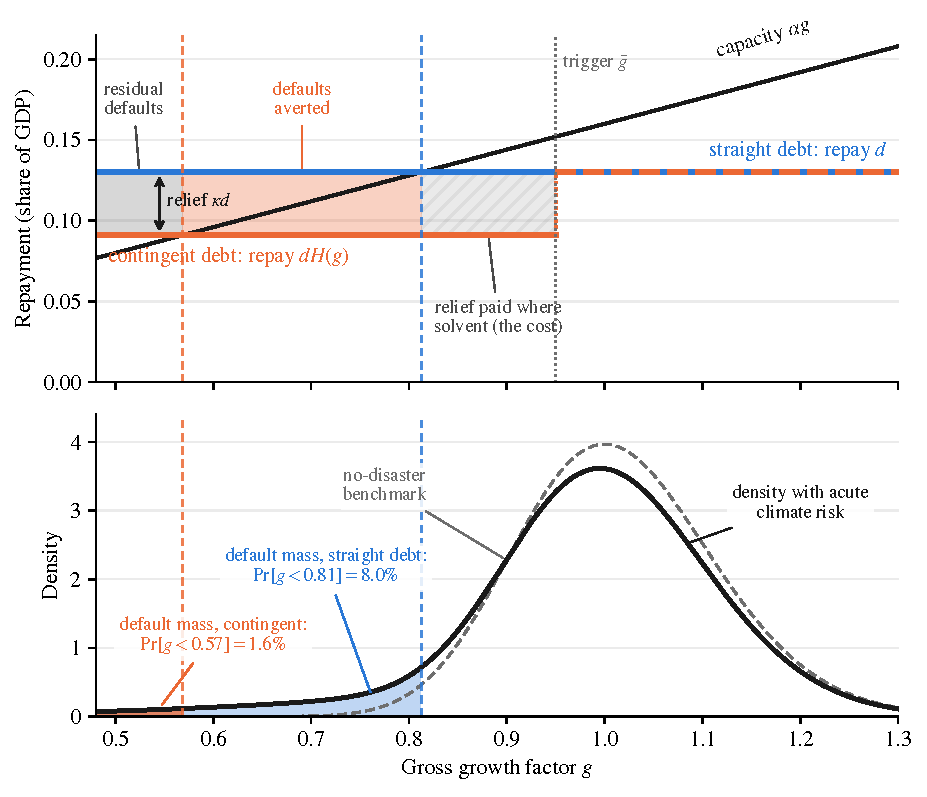
\includegraphics[width=0.88\linewidth]{fig1_loading.pdf}
\caption{How repayments load on left-tail states. \emph{Top panel:} with straight debt (face value $d=0.13$, surplus capacity $\alpha=0.16$), default occurs whenever the growth factor falls below $d/\alpha \approx 0.81$. A clause that cuts repayment by $\kappa=30\%$ in states below the trigger $\bar g = 0.95$ moves the default threshold down to $(1-\kappa)d/\alpha \approx 0.57$, splitting the relief into the three regions of the survival--payoff trade-off (Proposition~\ref{prop:interior_kappa}): relief that still ends in default, relief that converts default into survival, and relief given up in states in which the sovereign would have repaid anyway. \emph{Bottom panel:} the growth density under the acute-risk calibration of Section~\ref{sec:numerical} (lognormal growth plus Barro-style disaster jumps) attaches probability mass to those regions: the clause shrinks the default set's mass from $8.0\%$ to $1.6\%$. The dashed benchmark removes disasters; the thickened left tail is what makes the loading of repayments on left-tail states quantitatively first-order.}
\label{fig:intro_loading}
\end{figure}

The paper builds directly on the structural fiscal-limit framework of \textcite{CollardEtAl2015}---recently extended by \textcite{CollardHabibPanizzaRochet2024}---and on \textcite{Seghini2026}, who integrates emissions pathways and climate damages into the maximum sustainable borrowing calculation and shows that unmanaged damages eventually dominate transition costs, making coordinated mitigation fiscally essential. Relative to that baseline, this paper makes two contributions.

\emph{First, it generalizes the fiscal-limit object to a portfolio of state-contingent liabilities.} The sovereign issues a vector of instruments---straight bonds, GDP-linked bonds, disaster clauses, temperature-linked coupons---each with its own mapping from macro-climate states into repayments. Generalized MSB/MSD are defined over this portfolio, and the analysis provides implementable sufficient conditions under which contingent claims \emph{strictly} relax the fiscal limit relative to straight debt: the survival gain from removing repayments from default states must exceed the payoff given up in survival states.

\emph{Second, it extends the framework from chronic to acute physical risk.} In the NGFS taxonomy \parencite{NGFS2023}, chronic risk is the gradual erosion of growth by rising temperatures---the channel modeled by \textcite{Seghini2026} through a Dietz--Venmans damage function. Acute risk is the realization of discrete disasters. This paper introduces a Barro-style jump process for disasters \parencite{Barro2006}, allows the jump intensity to increase with cumulative emissions, and carries both through the quantitative exercise. This is precisely the risk category that disaster clauses are written on, so the extension is what makes the instrument analysis possible.

The quantitative section delivers magnitudes for both margins. At the baseline calibration, a GDP-linked clause raises the one-period MSB analogue by 10--12\% relative to straight debt while cutting the default probability at the issuance optimum from roughly 11\% to 3\%. The advantage is increasing in the rollover need---the clause \emph{costs} proceeds when debt is low and pays off strongly near the fiscal limit---increasing in the thickness of the left tail, exactly invariant to the level of surplus capacity (a homogeneity property of the fiscal-limit problem), and maximized at an interior level of contractual relief of around 20--30\% of face value. A disaster-triggered clause yields smaller gains (2--3\%) because its trigger is imperfectly correlated with the default set: basis risk, quantified. A temperature-linked coupon---a natural hedge against the global damage driver---adds value only when the coupling between global emissions realizations and domestic disaster intensity is strong; when the coupling is weak, the coupon's payoff noise dominates its insurance value in a one-period setting.

Two further channels are developed analytically but not calibrated, and it is important to state this scope limitation up front. A logistics-amplification channel maps global supply-chain disruptions into domestic output, surplus capacity, and sovereign risk premia, with production-network centrality governing exposure; the quantitative section varies the amplification parameter as a comparative static, but a full numerical solution and empirical calibration of this channel are beyond the scope of this paper. Likewise, a monetary block---climate-tilted collateral policy and asset purchases---is developed in Appendix~\ref{app:monetary} together with a simple comparative static on collateral haircuts; its equilibrium fixed point with long-maturity debt is left to future work.

The mechanisms studied here are fiscally first-order in the projections of fiscal institutions. The UK Office for Budget Responsibility, for example, now publishes scenario-based debt paths that attribute several percentage points of GDP of additional borrowing to climate-damage costs over multi-decade horizons (Figure~\ref{fig:obr_46}); parallel scenario work by the IMF and central banks treats climate damages and transition costs as joint, state-dependent objects \parencite{IMF2023FiscalMonitor,boe2024_climate_scenario_analysis}. And a growing empirical literature finds climate-related risk priced in sovereign bonds and reflected in ratings \parencite{ecb_wp3135_climate_pricing,ecb_wp3042_climate_ratings,zenios2021_bruegel_climate_debt,kling2025_climate_vulnerability_cost_debt}. Once climate risk is priced as a systematic component of sovereign risk rather than idiosyncratic disaster noise, the borrowing factor underpinning MSB/MSD is jointly determined by climate exposure, investor risk appetite, and liability design---which is what motivates treating debt management as an explicit climate-risk hedging problem.

\begin{figure}[!t]
  \centering
  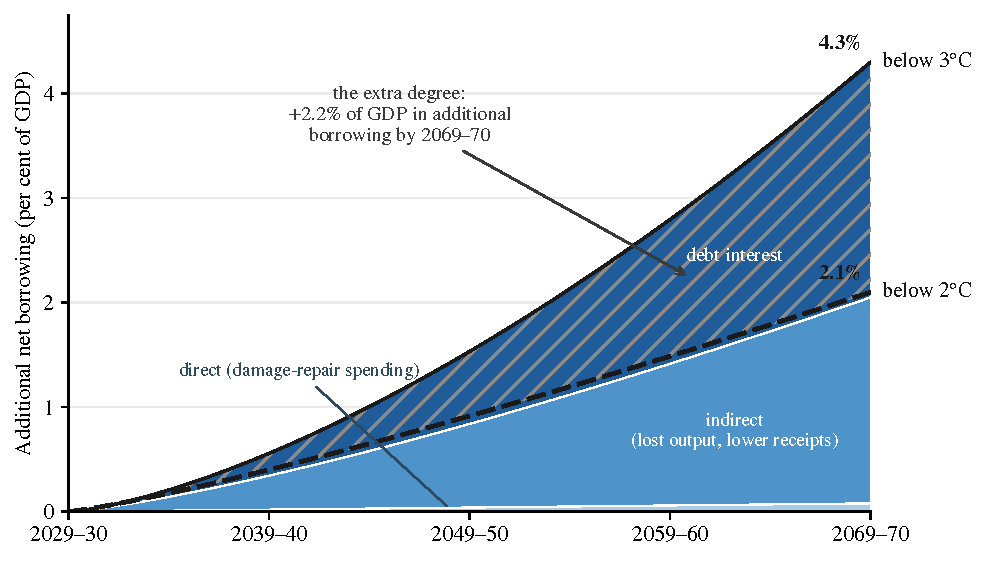
\includegraphics[width=0.92\linewidth]{fig2_climate_wedge.pdf}
  \caption{The fiscal cost of the extra degree. Additional public-sector net borrowing attributed to climate damage in the UK Office for Budget Responsibility's scenario analysis (author's stylized recreation of \cite{obr2025frs}, Chart 4.6). Shaded bands decompose the below-3$^\circ$C scenario into direct damage-repair spending, indirect revenue losses from lost output, and the debt interest that compounds on both; the dashed line is the below-2$^\circ$C total. The hatched wedge---roughly $2.2\%$ of GDP of annual borrowing by 2069--70---is the fiscal payoff to limiting warming. Climate damages are now routinely translated into long-horizon public-debt projections by fiscal institutions; this is the type of object that maps into the fiscal-limit calculations studied here.}
  \label{fig:obr_46}
\end{figure}

The paper proceeds as follows. Section~\ref{sec:baseline} summarizes the baseline fiscal-limit model with emissions and damages. Section~\ref{sec:extensions} develops the extensions that the paper quantifies: the acute-risk disaster process, the liability portfolio with generalized MSB/MSD, and the reduced-form logistics and premium channel; extensions that are analytical only (maturity, recovery, an endogenous risk-free rate, state-dependent volatility) are collected in Appendix~\ref{app:further}. Section~\ref{sec:results} states the analytical results. Section~\ref{sec:numerical} presents the quantitative illustration and comparative statics. Section~\ref{sec:conclusion} discusses design lessons and concludes. Appendix~\ref{app:pevc} develops the asset-market transmission to private equity and venture capital valuations, Appendix~\ref{app:monetary} the monetary block, and Appendix~\ref{app:proofs} the proofs.

\section{Baseline fiscal limits with emissions and damages}
\label{sec:baseline}

\textcite{Seghini2026} extends the Collard--Habib--Rochet framework (\cite{CollardEtAl2015}) by letting GDP growth depend on emissions paths (transition costs) and global cumulative emissions (damages). The core sustainability condition is
\begin{equation}
\frac{D_t}{Y_t} \le d_t^M,
\end{equation}
where $d_t^M$ is the fiscal limit (MSD), the debt-to-GDP ratio that maximizes borrowing proceeds (MSB). Default occurs when the face value of debt exceeds repayment resources:
\begin{equation}\label{eq:default_condition}
D_t - \alpha Y_t > B_t^M \quad \Longleftrightarrow \quad \frac{D_t}{Y_t} > \alpha + b_t^M,
\end{equation}
where $\alpha$ is the maximum primary surplus ratio (a fiscal-fatigue/Laffer constraint) and $b_t^M\equiv B_t^M/Y_t$ is maximum sustainable borrowing (\cite{Seghini2026}).

With risk-neutral pricing and a constant gross risk-free rate $R$, the promised gross return on sovereign debt satisfies
\begin{equation}\label{eq:pricing_basic}
R(d_t)\left(1-\mathrm{PD}(d_t)\right)=R.
\end{equation}

Equation (\ref{eq:pricing_basic}) is the key pricing identity that generates the borrowing-proceeds ``Laffer curve'' in the fiscal-limit framework. As face value issuance increases, default probability rises, and investors demand a higher promised gross return to break even. Borrowing proceeds therefore need not increase monotonically with promised repayments: beyond some point, additional face value is offset by sharply higher yields and a collapse in the present value of issuance revenue. MSB in (\ref{eq:MSB}) is exactly the peak of this proceeds curve, and MSD in (1) inherits its shape because sustainability is pinned down by the maximum resources the sovereign can raise subject to endogenous default risk.

Borrowing proceeds from issuing face value $d_t$ are $b(d_t)=d_t/R(d_t)$ and MSB is
\begin{equation}\label{eq:MSB}
b_t^M = \max_{d_t}\, b(d_t)=\max_{d_t}\frac{d_t}{R(d_t)}.
\end{equation}

A crucial step is the mapping from macro growth to default probability. In Seghini, growth is lognormal with an i.i.d.\ shock:
\begin{equation}\label{eq:growth_basic}
g_{t+1} \equiv \frac{Y_{t+1}}{Y_t}=H_{t+1}(\{E_t\}) e^{\mu_0+\varepsilon_{t+1}}, \quad \varepsilon_{t+1}\sim \mathrm{i.i.d.}\ \mathcal{N}(0,\sigma_0^2),
\end{equation}
where $H_{t+1}$ captures the effect of the emissions path on growth (transition costs). Seghini specifies
\begin{equation}\label{eq:seghini_eta}
H_{t+1}=\frac{\eta(E_{t+1})}{\eta(E_t)},\qquad \eta(E_t) = (c\bar E_1 + E_t)^{\beta},
\end{equation}
which implies (in relative emissions) a growth term $(\frac{c+e_{t+1}}{c+e_t})^{\beta}$ (\cite{Seghini2026}).

The emissions term in (\ref{eq:seghini_eta}) can be read as a multiplicative transition wedge on growth: holding the baseline shock fixed, changes in emissions reallocate resources and can temporarily depress measured output growth through adjustment costs. The crucial modeling move is that this wedge enters multiplicatively, so it scales the entire stochastic growth process rather than adding a deterministic amount. That formulation is convenient for mapping emissions policy into the default probability because it shifts the distribution of next-period output in a way that is directly comparable to damages and other growth wedges introduced later.

Importantly, Seghini adds an exponential damage function \`a la Dietz--Venmans:
\begin{equation}\label{eq:damage}
D(T_t)=\exp\!\left(-\frac{\rho}{2}T_t^2\right),\qquad T_t=\zeta C_t,
\end{equation}
with global cumulative emissions $C_t$, producing an additional multiplicative term in growth (\cite{DietzVenmans2019}). Her resulting growth equation (country $i$) can be written as
\begin{equation}\label{eq:seghini_growth_damage}
g_{i,t+1}= \exp\!\left(\mu_{0,i}+\varepsilon_{i,t+1}-\frac{\rho}{2}\left[(\zeta C_{t+1})^2-(\zeta C_t)^2\right]\right)\left(\frac{c+e_{i,t+1}}{c+e_{i,t}}\right)^{\beta_i}.
\end{equation}

The carbon budget enters as a hard constraint:
\begin{equation}\label{eq:carbon_budget}
\sum_{t\ge 0} E_t \le \bar E_0,
\end{equation}
which implies that emissions must eventually fall sufficiently, ensuring the ``no free-riding'' condition that bounds MSB (\cite{Blanchard2019}).

Seghini's quantitative results hinge on comparing fiscal limits under (i) coordinated transition, (ii) solitary transition, and (iii) global business-as-usual (BAU), showing that climate damages eventually dominate and coordination becomes fiscally essential. Two features of the baseline deserve emphasis for what follows. First, sovereign liabilities consist of a single instrument---one-period, non-interest-bearing debt rolled over each period---so the baseline model contains no ranking of debt instruments; instrument choice is precisely the margin this paper adds. Second, the damage channel is \emph{chronic} in the NGFS sense: damages accumulate smoothly with cumulative emissions, and there are no discrete disaster events. The assumptions delivering tractability (one-period debt, zero recovery, constant risk-free rate, i.i.d.\ lognormal growth) are flagged in \textcite{Seghini2026} as deliberate simplifications; the next section relaxes the ones this paper carries through to the quantitative exercise, and Appendix~\ref{app:further} discusses the remainder.

\section{Extensions to the baseline framework}
\label{sec:extensions}

\subsection{Transmission channels at a glance}
\label{subsec:channels}

The extensions are best understood as links in a single transmission chain running from the global climate state to the fiscal limit. The chain begins with the global climate state itself: cumulative emissions erode trend growth---the chronic-risk channel already present in the baseline---and, in this paper, also raise the intensity of discrete disaster jumps, the acute-risk margin developed in Section~\ref{subsec:acute}. Climate shocks need not strike domestic territory to matter fiscally. Shocks that hit trade routes, ports, and suppliers abroad reduce domestic output through a logistics wedge whose size depends on the country's production-network centrality and import dependence (Section~\ref{subsec:logistics}); an external disruption therefore resembles a domestic macro shock in that it compresses the tax base without any local disaster occurring. Both channels also operate on the fiscal side directly, reducing the politically feasible primary surplus in stressed states and thereby adding a fiscal-fatigue margin to the output effects. The liability portfolio then maps realized macro-climate states into contractual repayments, and instrument design consists precisely in choosing this mapping (Section~\ref{subsec:portfolio}). Default occurs when contractual repayments exceed state-contingent capacity; the resulting default probability, together with climate and logistics exposure, feeds the sovereign premium, which prices new issuance and hence determines the fiscal limit. Finally, policy enters at the pricing stage: collateral eligibility and asset purchases can lower premia on specific instruments, interacting with the repayment mapping and the premium just described. This monetary interface is developed in Appendix~\ref{app:monetary}, where the same one-period apparatus is used for a comparative static on collateral haircuts.

The quantitative exercise in Section~\ref{sec:numerical} operationalizes every link of this chain except the policy interface in a one-period setting; the appendices treat the monetary interface (Appendix~\ref{app:monetary}) and the asset-pricing spillover to private capital (Appendix~\ref{app:pevc}).

\subsection{Acute physical risk: disasters as jumps}
\label{subsec:acute}

In the baseline, the i.i.d.\ lognormal shock is chosen for tractability and pseudo-analytic results (\cite{Seghini2026}). However, acute physical risk is better represented by fat-tailed disasters (\cite{Barro2006}; \cite{Mallucci2022}). If disasters arrive as jumps $J_{t+1}\le 0$ with intensity $\lambda_t$ increasing in temperature,
\begin{equation}\label{eq:jump_growth}
\log g_{t+1} = \mu_t + \varepsilon_{t+1}+J_{t+1},\quad \mathbb{P}(J_{t+1}\neq 0|\mathcal{F}_t)=\lambda(T_t),
\end{equation}
then the default probability is more sensitive to climate damages than in the lognormal case, because the left tail thickens. This tends to lower MSD in BAU relative to coordinated transition more dramatically than in the baseline, strengthening Seghini's qualitative conclusion while altering the timing and optimal policy mix. The mapping $\lambda(T_t)$ ties the arrival intensity of acute events to the same global state variable---cumulative emissions---that drives chronic damages, so the two NGFS risk categories share a common driver. Both the jump process and a state-dependent $\lambda$ are carried through the quantitative exercise in Section~\ref{sec:numerical}; the specification with disaster clustering over time (serially correlated intensity) interacts with maturity structure and is discussed in Appendix~\ref{app:further}.

\subsection{A portfolio of sovereign liabilities and generalized fiscal limits}
\label{subsec:portfolio}

I now generalize MSB/MSD to a sovereign liability portfolio. Let the government issue $K$ instruments with face values (or notional shares) collected in a vector $\bm{d}_t=(d^1_t,\dots,d^K_t)$ as ratios to GDP. All instruments are one-period securities, maturing next period; maturity extension is a separate margin, discussed in Appendix~\ref{app:further}. Instrument $k$ has a state-contingent gross payoff function $\Pi^k_{t+1}(\omega_{t+1})$ per unit of notional, where $\omega_{t+1}$ summarizes macro states (growth, temperature, disaster occurrence, etc.). Let the market price per unit notional be $q^k_t$, so proceeds are $b^k_t=d^k_t q^k_t$, and total proceeds are
\begin{equation}
b_t(\bm{d}_t)=\sum_{k=1}^K d^k_t q^k_t.
\end{equation}
Total contractual repayment due next period (as a ratio to $Y_t$) is
\begin{equation}\label{eq:due_total}
\Delta_{t+1}(\omega_{t+1};\bm{d}_t)=\sum_{k=1}^K d^k_t \Pi^k_{t+1}(\omega_{t+1}).
\end{equation}

I preserve the ``excusable default'' spirit: default occurs when required repayment exceeds resources. However, resources can now include (i) primary surplus capacity and (ii) instrument-specific state-contingent relief (already in $\Pi^k$), plus (iii) disaster-recovery inflows if modeled as insurance. Let $g_{t+1}\equiv Y_{t+1}/Y_t$ denote the gross growth factor. Default occurs if
\begin{equation}\label{eq:default_multi}
\Delta_{t+1}(\omega_{t+1};\bm{d}_t) > (\alpha_t + b_{t+1}^M)\, g_{t+1}.
\end{equation}
Thus, the default probability is
\begin{equation}\label{eq:PD_multi}
\mathrm{PD}(\bm{d}_t)=\mathbb{P}\left(\Delta_{t+1}(\omega_{t+1};\bm{d}_t) > (\alpha_t + b_{t+1}^M)\, g_{t+1}\ \big|\ \mathcal{F}_t\right).
\end{equation}

Let investors price instruments with a stochastic discount factor $M_{t+1}$ that depends on global risk and climate states. Then
\begin{equation}\label{eq:pricing_sdf}
q^k_t = \mathbb{E}_t\left[M_{t+1}\,\Pi^k_{t+1}(\omega_{t+1})\,\mathbf{1}\{\tau>t+1\} + M_{t+1}\,\mathcal{R}^k_{t+1}\,\mathbf{1}\{\tau=t+1\}\right],
\end{equation}
where $\tau$ is the default time and $\mathcal{R}^k_{t+1}$ is recovery conditional on default. This nests Seghini's risk-neutral, constant-$R$ pricing when $M_{t+1}=1/R$ and recoveries are zero (\cite{Seghini2026}).

Define generalized MSB as maximum proceeds achievable by choosing the instrument mix subject to feasibility and a carbon budget:
\begin{equation}\label{eq:MSB_general}
b_t^M = \max_{\bm{d}_t\in \mathcal{D}_t}\ b_t(\bm{d}_t)
\end{equation}
subject to the induced default probability being consistent with market pricing and with the continuation borrowing capacity $b_{t+1}^M$ (a fixed-point condition analogous to \textcite{CollardEtAl2015}). The generalized fiscal limit (MSD) can be defined as the set of debt vectors that achieve MSB, or as the maximum of a chosen scalar aggregator of debt (e.g.\ weighted face value) subject to not exceeding MSB. A natural scalar is total expected repayment in the no-default state:
\begin{equation}\label{eq:MSD_scalar}
d_t^M \equiv \max_{\bm{d}_t\in \mathcal{D}_t} \sum_{k=1}^K d^k_t \bar \Pi^k \quad \text{s.t.}\quad b_t(\bm{d}_t)\le b_t^M,
\end{equation}
where $\bar\Pi^k$ is a normalization (e.g.\ promised payoff in the baseline state).

I consider four instruments, all of which appear in the quantitative exercise. \emph{Instrument 1: straight debt.} $\Pi^1_{t+1}=1$, a one-period, non-interest-bearing security with face value normalized. This corresponds to Seghini's baseline (\cite{Seghini2026}).

\emph{Instrument 2: GDP-linked bonds}, which pay less in low-output states:
\begin{equation}\label{eq:gdp_linked}
\Pi^2_{t+1}= 1 + \kappa_g\left(\frac{g_{t+1}}{\bar g}-1\right),
\end{equation}
with $\kappa_g\in(0,1)$ and $\bar g$ a reference growth level. When $g_{t+1}$ is low, repayment falls, reducing default probability (\cite{BorenszteinMauro2004}; \cite{ChamonMauro2006}; \cite{KimOstry2018}). The quantitative section works with the threshold (clause) version $\Pi_{t+1} = 1-\kappa\,\mathbf{1}\{g_{t+1}<\bar g\}$, which is closer to contractual practice.

\emph{Instrument 3: disaster clauses.} The clause triggers a payment reduction (in practice, a maturity extension or coupon suspension) if a disaster indicator $Z_{t+1}\in\{0,1\}$ turns on. In one-period form,
\begin{equation}\label{eq:cat_clause}
\Pi^3_{t+1}=1-\kappa_Z Z_{t+1}, \quad \kappa_Z\in(0,1),
\end{equation}
with $Z_{t+1}=1$ when verified disaster losses exceed a threshold (\cite{WorldBankCatBonds}). This is the CRDC payoff in reduced form.

\emph{Instrument 4: temperature-linked (cumulative-emissions-linked) coupons.} Because Seghini's damage term is driven by global cumulative emissions $C_t$ (\cite{Seghini2026}), a natural hedge is an instrument whose repayments fall when emissions growth overshoots a reference path:
\begin{equation}\label{eq:temp_linked}
\Pi^4_{t+1}= 1-\kappa_T\left(\frac{\Delta C_{t+1}-\overline{\Delta C}}{\overline{\Delta C}}\right),
\end{equation}
where $\Delta C_{t+1} = C_{t+1}-C_t$, $\kappa_T>0$, and $\overline{\Delta C}$ is the reference emissions increment, so the expected payoff is one on the reference path. This instrument pays insurance in precisely the states where damages accelerate (and where BAU becomes fiscally explosive). Its value, however, hinges on how tightly global emissions realizations are coupled to domestic default states at the relevant horizon---a question Section~\ref{subsec:temp_sim} answers quantitatively. A fifth design---resilience bonds indexed to verified adaptation capital---pairs naturally with the collateral policy discussed in the monetary block and is presented in Appendix~\ref{app:monetary}.

A central reason these instruments remain underused, despite their theoretical appeal, is that they can carry novelty and ambiguity premia, as well as concerns over measurement, verification, and basis risk in triggers (\cite{igan2021_premia_scdi}; \cite{volz2022_state_contingent_debt}; \cite{pina2022_scgd_database}). This paper therefore treats instrument choice as a joint problem of (i) shifting repayments out of default-relevant states, and (ii) designing triggers and payoffs that are sufficiently transparent to limit premia. The resulting comparative statics clarify when the reduction in default probability dominates any ex ante pricing discount, delivering a strict relaxation of MSB/MSD.

\subsection{Logistics disruption, surplus capacity, and sovereign premia}
\label{subsec:logistics}

Climate shocks do not only destroy local capital; they disrupt trade routes, ports, shipping, and intermediate input supply, creating production-network amplification (\cite{AcemogluCarvalho2012}; \cite{Carvalho2014}). These disruptions matter for fiscal limits through two mechanisms: (i) they depress domestic output and tax bases, and (ii) they raise sovereign risk premia via investor perceptions of macro fragility.

Let $\ell_{i,t}\ge 0$ denote a logistics disruption wedge for country $i$ that scales effective output. Suppose
\begin{equation}\label{eq:logistics_wedge}
\log \ell_{i,t+1}= \varphi_i Z_{t+1} + \psi_i \, \mathrm{NetCen}_i \, Z^{\mathrm{global}}_{t+1} + u_{i,t+1},
\end{equation}
where $\mathrm{NetCen}_i$ measures production-network centrality (or trade-route exposure), $Z^{\mathrm{global}}$ is a global logistics shock (e.g.\ a major shipping choke-point disruption), and $u$ is idiosyncratic noise. Then modify Seghini's growth by
\begin{equation}\label{eq:growth_with_logistics}
g_{i,t+1}= g^{\mathrm{Seghini}}_{i,t+1}\cdot \exp(-\ell_{i,t+1}),
\end{equation}
where $g^{\mathrm{Seghini}}_{i,t+1}$ is given by \eqref{eq:seghini_growth_damage}. This nests Seghini when $\ell\equiv 0$. The composite parameter $\psi_i\,\mathrm{NetCen}_i$ is what the quantitative section varies as a single amplification scalar $\psi$: it is a reduced-form loading of domestic output on global logistics shocks, and its empirical counterpart is a centrality measure from input-output or trade-network data (eigenvector or Katz--Bonacich centrality, import dependence in critical intermediates), which the physical-risk propagation literature shows to govern the pass-through of remote disasters to domestic activity (\cite{BarrotSauvagnat2016}; \cite{inoue_todo2019_supply_chain}; \cite{boehm2019_input_linkages}).

One clarification is important, because this paper elsewhere emphasizes departures from i.i.d.\ growth: specification \eqref{eq:growth_with_logistics} does \emph{not} by itself relax the i.i.d.\ assumption. If $Z^{\mathrm{global}}_{t+1}$ and $u_{i,t+1}$ are i.i.d., the wedge $\ell_{i,t+1}$ is i.i.d.\ too, and its role is to thicken the left tail of the within-period growth distribution rather than to introduce serial dependence. Serial dependence---clustered disasters, multi-year reconstruction, persistent disruption---requires an autocorrelated intensity or wedge process, which interacts with maturity structure and is discussed in Appendix~\ref{app:further}. The quantitative exercise below is therefore a statement about tail thickness, not persistence.

In Seghini, $\alpha$ is constant and calibrated to historical maxima (\cite{Seghini2026}). But climate and logistics disruptions alter political feasibility and revenue capacity. Let
\begin{equation}\label{eq:alpha_endog}
\alpha_{i,t} = \bar \alpha_i - \chi_T D_T(T_t) - \chi_\ell \ell_{i,t},
\end{equation}
where $D_T(T_t)$ is a damage index increasing in $T_t$ and $\chi_T,\chi_\ell>0$. This captures ``fiscal fatigue'' worsening in stressed states (\cite{GhoshEtAl2013}). The quantitative exercise holds $\alpha$ constant---the homogeneity result in Section~\ref{subsec:gains} shows that the \emph{relative} gains from contingency are invariant to the level of $\alpha$---so \eqref{eq:alpha_endog} should be read as an analytical extension whose quantitative implementation is left to future work.

Let sovereign pricing incorporate a premium $\pi_{i,t}$ so that $R_{i,t}=R_{f,t}\exp(\pi_{i,t})$. Model
\begin{equation}\label{eq:premium}
\pi_{i,t} = \theta_d\,\mathrm{PD}_{i,t} + \theta_T T_t + \theta_\ell \ell_{i,t} + \theta_x \mathrm{FXFrag}_{i,t}.
\end{equation}
Each term has a distinct economic rationale and a signed coefficient. The first term is default compensation: under risk-neutral pricing the premium must rise one-for-one with expected default losses, so $\theta_d>0$, and in the presence of risk aversion $\theta_d$ exceeds the actuarial level. The second term captures the pricing of \emph{systematic} climate exposure: if damages are driven by the global state $T_t$, they cannot be diversified away, so investors demand compensation beyond expected losses, implying $\theta_T>0$ for damage-exposed issuers (\cite{ecb_wp3135_climate_pricing}). The third term reflects logistics fragility: a country whose output is exposed to supply-chain disruption has a more fragile tax base for a given default probability, and the empirical sovereign-risk literature finds such macro-fragility characteristics priced over and above model-implied PD, so $\theta_\ell>0$. The fourth term, $\mathrm{FXFrag}_{i,t}$---external vulnerability and currency mismatch of the sovereign balance sheet---raises the loss given stress and the likelihood of self-fulfilling runs, so $\theta_x>0$ (\cite{Mallucci2022}). This creates a feedback loop: climate and logistics raise premia, premia tighten fiscal limits, tighter limits constrain adaptation and transition finance, increasing future damages. These reduced-form sensitivities could be parameterized in future empirical work using spread responses to climate and logistics shocks; the present paper does not estimate them, and in the simulations the risk-free rate and premium are held constant except where noted.

Sovereign premia also transmit to the discount rates applied to private capital---private equity and venture capital (PE/VC) valuations in particular---linking sovereign sustainability to international asset markets. Because that channel is not used in the quantitative exercise, it is developed in Appendix~\ref{app:pevc}.

\section{Analytical results: when contingent instruments relax fiscal limits}
\label{sec:results}

I now show that state-contingent instruments can strictly increase MSB/MSD relative to straight debt, under implementable conditions.

Consider a one-period setting to parallel Seghini. Let $k=1$ be straight debt with payoff $\Pi^1_{t+1}=1$. Let $k=2$ be a contingent instrument with payoff $\Pi^2_{t+1}=1-\kappa \cdot \mathbb{1}\{g_{t+1}<\bar g\}$, i.e.\ it reduces repayment in bad states (GDP-linked or disaster-linked). Assume investors price with a state-independent $R_f$ for clarity and recovery is zero. Consider issuing a small share $\epsilon$ of instrument 2 replacing instrument 1 while keeping total face value constant.

Let $\Delta_{t+1}(\epsilon) = d\big[(1-\epsilon)\Pi^1_{t+1}+\epsilon \Pi^2_{t+1}\big]$. Then the default event is
\begin{equation}
\Delta_{t+1}(\epsilon) > (\alpha + b_{t+1}^M)\, g_{t+1}.
\end{equation}
Because $\Pi^2_{t+1}\le \Pi^1_{t+1}$ in bad states and equals it in good states, the set of $\omega_{t+1}$ leading to default weakly shrinks when $\epsilon$ increases. Therefore,
\begin{equation}\label{eq:PD_decreases}
\frac{\partial \mathrm{PD}}{\partial \epsilon}\le 0,
\end{equation}
with strict inequality whenever the threshold region has positive probability mass.

Borrowing proceeds are
\begin{equation}
b(\epsilon)= d\left[(1-\epsilon)q^1 + \epsilon q^2\right].
\end{equation}
With risk-neutral pricing, $q^k=\mathbb{E}\left[\Pi^k_{t+1}\mathbb{1}\{\tau>t+1\}\right]/R_f$.
If adding contingency reduces PD sufficiently, the survival-weighted payoff can rise even if the instrument pays less in bad states. A sufficient condition for $b'(\epsilon)>0$ at $\epsilon=0$ is
\begin{equation}\label{eq:sufficient_condition}
\underbrace{\frac{\partial}{\partial \epsilon}\mathbb{E}\big[\mathbf{1} \{\tau>t+1\}\big]\Big|_{\epsilon=0}}_{\text{survival gain}}
>\underbrace{\kappa \cdot \mathbb{P}(g_{t+1}<\bar g,\ \tau>t+1)\Big|_{\epsilon=0}}_{\text{payoff reduction in survival states}}.
\end{equation}
Condition \eqref{eq:sufficient_condition} is intuitive: if contingency meaningfully reduces default probability in precisely the states where default would otherwise occur, it increases the value of being repaid at all, raising proceeds.

In Seghini, the MSB recursion is linear in $(\alpha+b^M_{t+1})$ with a constant borrowing factor $\gamma e^{\mu_0}/R$ (\cite{Seghini2026}). With instrument choice, the borrowing factor becomes a functional of the payoff mapping:
\begin{equation}\label{eq:borrowing_factor_general}
b_t^M = \max_{\bm{d}_t}\ \frac{e^{\mu_t}}{R_{f,t}}\ \Gamma(\bm{d}_t;\sigma_t,\text{tails})\ (\alpha_t+b_{t+1}^M)\, \mathbb{E}_t[H_{t+1} \mid \bm{d}_t],
\end{equation}
where $\Gamma$ is an effective borrowing factor that increases when payoffs reduce repayments in the left tail (default states). Thus, the instrument mix is a lever that modifies the financial amplification channel, not merely a funding choice.

Because damages accelerate with $(\zeta C_t)^2$ in Seghini's damage term (\cite{Seghini2026}), BAU implies an increasing drift toward low-growth states. A temperature-linked payoff \eqref{eq:temp_linked} explicitly reduces repayment as $\Delta C$ rises, transferring resources from BAU-bad states to BAU-good states. Even if such instruments command a premium (lower $q$) in normal times, they can stabilize fiscal limits by preventing the sharp MSD decline that Seghini finds under BAU. This reasoning yields two predictions, which should be read as conjectures that the quantitative section examines in a one-period setting and that a full dynamic implementation would test more sharply. First, countries with higher exposure to global damages (higher $\theta_T$ in \eqref{eq:premium}) should benefit more---in terms of fiscal-limit stabilization---from temperature-linked clauses than from GDP-linked clauses alone, because the underlying state variable is global and persistent; Section~\ref{subsec:temp_sim} shows that the strength of the coupling between the global state and domestic default states is exactly what determines the sign of the temperature-linked gain. Second, under \eqref{eq:logistics_wedge}--\eqref{eq:growth_with_logistics}, countries with high network centrality experience larger output losses when global logistics disruptions occur, so the fiscal value of well-targeted contingency should be increasing in logistics-network centrality and import dependence, holding local disaster risk constant; Section~\ref{subsec:gains} confirms this comparative static in $\psi$. The corresponding results for monetary support (collateral and purchases) are stated and discussed in Appendix~\ref{app:monetary}.

\section{Quantitative illustration: how much do contingent claims relax the fiscal limit?}
\label{sec:numerical}

\subsection{Purpose and design}
\label{subsec:design}

This section quantifies the paper's mechanism in a transparent one-period environment. Three scope statements up front. First, the exercise is a numerical \emph{illustration}, not an empirical calibration to a specific country: parameters are chosen to be defensible orders of magnitude (Table~\ref{tab:params}), and the outputs of interest are comparative statics---percentage gains in the fiscal-limit analogue across instruments and environments---rather than levels. Second, \emph{the gross risk-free rate $R_f$ is held constant throughout the simulations}; the general-equilibrium determination of $R_f$ is discussed in Appendix~\ref{app:further}. Third, the exercise sets the continuation borrowing capacity $b^M_{t+1}$ to zero, so that repayment capacity is $\alpha g$ alone; this makes the levels conservative (they omit the value of future market access) without affecting the cross-instrument comparisons that are the object of interest.

Throughout this section, $g$ denotes the gross output growth factor $Y_{t+1}/Y_t$ over one model period, consistent with its use in Sections~\ref{sec:baseline}--\ref{sec:results}. For face value $d$ and a payoff mapping $H(g)$, repayment due is $dH(g)$ and fiscal capacity is $\alpha g$. Default occurs if
\begin{equation}\label{eq:default}
dH(g) > \alpha g .
\end{equation}
Assume risk-neutral pricing with gross risk-free rate $R_f$. The issuance price per unit face value is
\begin{equation}\label{eq:iss_price}
q(d) = \frac{\mathbb{E}\big[H(g)\mathbf{1}\{dH(g)\le \alpha g\}\big]}{R_f},
\end{equation}
so proceeds are $b(d)=dq(d)$. The maximum of $b(d)$ over $d$ is the numerical analogue of MSB: it captures the peak amount the sovereign can raise once default risk and pricing are internalized.

Given i.i.d.\ draws $\{g^{(n)}\}_{n=1}^N$, the Monte Carlo estimators are
\begin{align}
\widehat{q}_N(d;\chi) &= \frac{1}{R_f}\cdot \frac{1}{N}\sum_{n=1}^N H\!\left(g^{(n)},\chi\right)\,
\mathbf{1}\!\left\{d\,H\!\left(g^{(n)},\chi\right)\le \alpha g^{(n)}\right\}, \label{eq:qhat}\\
\widehat{b}_N(d;\chi) &= d\,\widehat{q}_N(d;\chi), \qquad
\widehat{PD}_N(d;\chi)=\frac{1}{N}\sum_{n=1}^N \mathbf{1}\!\left\{d\,H\!\left(g^{(n)},\chi\right)> \alpha g^{(n)}\right\}, \label{eq:bhpdh}
\end{align}
where $\chi$ collects contract parameters. The numerical MSB analogue is
\begin{equation}
\widehat{b}^M_N(\chi)=\max_{d\in\mathcal{D}}\widehat{b}_N(d;\chi), \qquad
\widehat{d}^*_N(\chi)\in\arg\max_{d\in\mathcal{D}}\widehat{b}_N(d;\chi),
\label{eq:msbhat}
\end{equation}
for a grid $\mathcal{D}=[0,0.40]$ in steps of $0.001$. Consistency of these estimators is established in Appendix~\ref{app:proofs}. All results use $N=200{,}000$ draws and a fixed seed; the replication code is archived with the paper.

Growth over the period is modeled as
\begin{equation}\label{eq:output}
g = \exp(\mu+\varepsilon+J)\cdot \exp(-\psi L),
\end{equation}
where $\varepsilon\sim \mathcal{N}(0,\sigma^2)$ is the baseline growth shock; $J\le 0$ is a rare-disaster jump, active with probability $p_{\text{dis}}$ and with magnitude drawn from an exponential distribution with mean $|\mathbb{E}[J]|$ (an operational version of \eqref{eq:jump_growth}); and $L\ge 0$ is a logistics disruption wedge, active with probability $p_{\text{log}}$ with exponential magnitude of mean $\mathbb{E}[L]$. The scalar $\psi\ge 0$ is the logistics amplification of Section~\ref{subsec:logistics}: it stands in for the composite loading $\psi_i\,\mathrm{NetCen}_i$, so sweeping $\psi$ traces out countries of increasing production-network centrality.

I compare the payoff mappings
\begin{align}
H_{\text{straight}}(g) &= 1, \label{eq:Hstraight}\\
H_{\text{GDP}}(g;\kappa,\bar g) &= 1-\kappa\,\mathbf{1}\{g<\bar g\}, \label{eq:Hgdp}\\
H_{\text{DIS}}(Z;\kappa_Z) &= 1-\kappa_Z Z, \qquad Z\in\{0,1\}, \label{eq:Hdis}
\end{align}
plus the temperature-linked coupon \eqref{eq:temp_linked} in Section~\ref{subsec:temp_sim}. The GDP clause targets the endogenous left tail directly; the disaster clause targets an observable event trigger ($Z=1$ when the jump is active) and therefore illustrates basis risk relative to default states. Two implementable trade-offs are explored: generosity ($\kappa$) increases survival in bad states but reduces payoffs conditional on survival; and the trigger ($\bar g$) trades off targeting (low basis risk relative to default states) versus frequent activation.

\subsection{Calibration}
\label{subsec:calibration}

Table~\ref{tab:params} reports the parameter values, their annual equivalents, and their provenance. The model period is five years, following Seghini's periodization; because the model is solved at that frequency, all values in the table are reported both per period and in annual terms.

\begin{table}[t]
\centering
\caption{Calibration of the numerical illustration. The model period is 5 years (Seghini's periodization); annual equivalents are reported for comparability.}
\label{tab:params}
\resizebox{\textwidth}{!}{%
\begin{tabular}{@{}llll@{}}
\toprule
Parameter & Per 5-yr period & Annual equivalent & Source / rationale \\ \midrule
Risk-free gross rate $R_f$ & $1.08$ & $1.55\%$/yr & long-run real safe rate (\cite{Blanchard2019}) \\
Fiscal capacity $\alpha$ & $0.16$ & $3.2\%$ of GDP/yr & max primary surplus (\cite{GhoshEtAl2013}; \cite{CollardEtAl2015}) \\
Mean log growth $\mu$ & $0.01$ & $0.2\%$/yr & conservative damage-adjusted trend \\
Growth volatility $\sigma$ & $0.10$ & $4.5\%$/yr & pooled 5-yr growth dispersion, AEs \\
Disaster prob.\ $p_{\text{dis}}$ & $0.15$ & $3.2\%$/yr hazard & \cite{Barro2006}; \cite{Mallucci2022} \\
Disaster size $|\mathbb{E}[J]|$ & $0.25$ (exponential) & mean loss $25\%$ & \cite{Barro2006} disaster sizes \\
Logistics prob.\ $p_{\text{log}}$ & $0.08$ & $1.65\%$/yr hazard & 1--2 global disruptions/decade (\cite{UNCTAD2022}) \\
Logistics wedge $\mathbb{E}[L]$ & $0.06$ & $6\%$ output wedge & network propagation (\cite{inoue_todo2019_supply_chain}) \\
GDP clause $(\kappa,\bar g)$ & $(0.30,\;0.95)$ & --- & CRDC-scale deferral (\cite{icma2022_crdc_chairs_summary}) \\
Disaster clause $\kappa_Z$ & $0.35$ & --- & 2-yr service suspension $\approx 40\%$ of 5-yr service \\
Temperature coupon $\kappa_T$ & $0.30$ & --- & symmetric coupon step, Section~\ref{subsec:temp_sim} \\
Logistics amplification $\psi$ & $\{0,\dots,3\}$ & --- & centrality loading, swept as comparative static \\
Face-value grid $\mathcal{D}$ & $[0,\,0.40]$, step $0.001$ & --- & spans the post-peak region for all $\alpha$ considered \\
\bottomrule
\end{tabular}}
\end{table}

Three calibration choices need explanation. First, the clause parameters: $\kappa=0.30$ means the clause forgives (or defers beyond the period) 30\% of the repayment due when the trigger is hit, and $\kappa\in[0.1,0.8]$ is swept in Section~\ref{subsec:kappa}; the anchor is the scale of actual CRDCs, under which a two-year suspension of debt service amounts to roughly 40\% of the service due within a five-year window. The trigger $\bar g = 0.95$ activates the clause when output over the period falls 5\% or more below its starting level---a severe-recession/disaster region. Second, the units of $d$: because debt is one-period and matures within the period, $d$ is the \emph{face value due within the current five-year period} as a share of GDP, not the total stock of public debt. With continuation borrowing set to zero, the sustainable $d$ is bounded by within-period surplus capacity, which is why the proceeds curves peak near $d\approx 0.13$--$0.15$ (about 2.6--3\% of GDP per year of maturing debt service). This is the one-period analogue of the rollover need, not a claim that fiscal limits are 13\% of GDP; in the full recursion, capacity is $\alpha+b^M_{t+1}$ and the corresponding MSD is an order of magnitude larger, as in \textcite{CollardEtAl2015} and \textcite{Seghini2026}. Third, disaster sizes are exponentially distributed rather than fixed, matching the archived replication code; this makes the left tail heavier than a fixed-jump specification and is the natural operationalization of ``fatter-tailed'' acute risk.

\subsection{Proceeds and default risk}
\label{subsec:laffer}

Figure~\ref{fig:proceeds} plots issuance proceeds $b(d)$ against face value $d$ for straight debt and the GDP clause, at $\psi=0$ and $\psi=1.5$; Figure~\ref{fig:pd} shows the associated default probabilities. Contracts are distinguished by color (blue: straight; orange: GDP clause) and the logistics scenario by line style (solid: $\psi=0$; dashed: $\psi=1.5$).

With straight debt, proceeds rise nearly linearly while default is rare, peak at $\widehat d^*\approx 0.13$, and collapse as default becomes pervasive. The contingent clause shifts the peak up and to the right ($\widehat d^*\approx 0.15$): by cutting repayments in states below $\bar g$, it removes exactly the marginal default states that destroy issuance value near the straight-debt peak. At the respective optima, the clause raises peak proceeds by 10.5\% ($\psi=0$) while cutting the default probability from 10.8\% to 3.0\% (Table~\ref{tab:msb_contracts}).

The $\psi=1.5$ curves lie almost on top of the $\psi=0$ curves, and this deserves comment rather than concealment: at the baseline parameterization the \emph{unconditional} logistics drag is $p_{\text{log}}\times\psi\times\mathbb{E}[L]\approx 0.7\%$ of output, so moderate amplification barely moves the proceeds curve even though it visibly worsens tail outcomes conditional on disruption. The economically relevant comparative static is therefore the systematic sweep of $\psi$ in Table~\ref{tab:msb_contracts} and Figure~\ref{fig:msb_vs_psi}, where the erosion of straight-debt capacity and the stabilizing role of contingency emerge monotonically.

\begin{figure}[t]
\centering
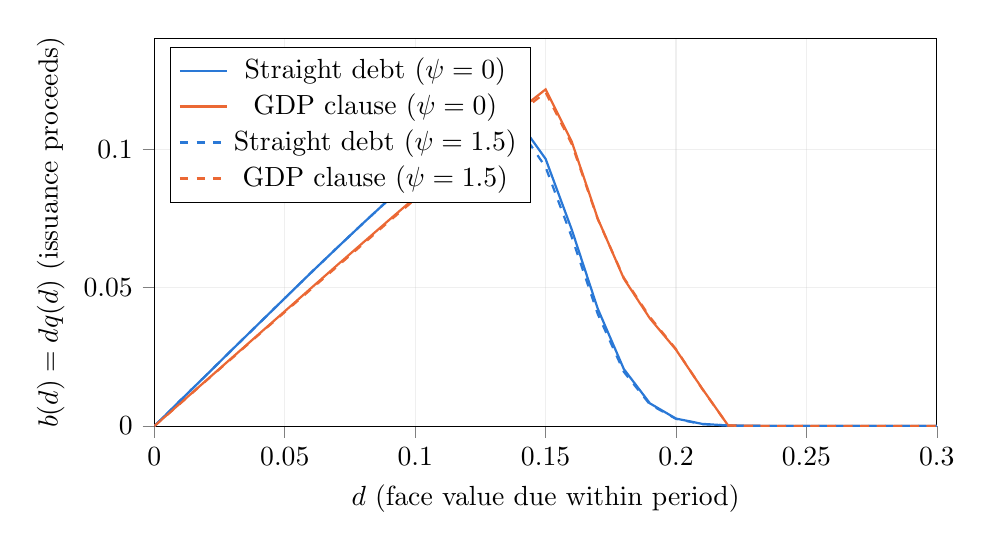
\begin{tikzpicture}
\begin{axis}[
  width=0.95\linewidth,
  height=6.5cm,
  xlabel={$d$ (face value due within period)},
  ylabel={$b(d)=d q(d)$ (issuance proceeds)},
  legend style={at={(0.02,0.98)},anchor=north west},
  xmin=0, xmax=0.30, ymin=0, ymax=0.14,
  xtick={0,0.05,0.10,0.15,0.20,0.25,0.30},
  scaled x ticks=false, scaled y ticks=false,
  tick label style={/pgf/number format/fixed},
  x tick label style={/pgf/number format/fixed,/pgf/number format/precision=2},
  y tick label style={/pgf/number format/fixed,/pgf/number format/precision=2},
  grid=major, major grid style={opacity=0.25},
  tick align=outside, tick pos=left,
]
\addplot[vizblue, thick] coordinates {(0.00,0.0000) (0.01,0.0093) (0.02,0.0185) (0.03,0.0278) (0.04,0.0370) (0.05,0.0462) (0.06,0.0554) (0.07,0.0644) (0.08,0.0733) (0.09,0.0820) (0.10,0.0904) (0.11,0.0983) (0.12,0.1055) (0.13,0.1108) (0.14,0.1098) (0.15,0.0966) (0.16,0.0711) (0.17,0.0424) (0.18,0.0206) (0.19,0.0082) (0.20,0.0027) (0.21,0.0008) (0.22,0.0002) (0.23,0.0001) (0.24,0.0000) (0.25,0.0000) (0.26,0.0000) (0.27,0.0000) (0.28,0.0000) (0.29,0.0000) (0.30,0.0000)};
\addlegendentry{Straight debt ($\psi=0$)}
\addplot[vizorange, thick] coordinates {(0.00,0.0000) (0.01,0.0083) (0.02,0.0166) (0.03,0.0249) (0.04,0.0332) (0.05,0.0415) (0.06,0.0498) (0.07,0.0581) (0.08,0.0663) (0.09,0.0745) (0.10,0.0826) (0.11,0.0907) (0.12,0.0987) (0.13,0.1066) (0.14,0.1143) (0.15,0.1217) (0.16,0.1029) (0.17,0.0750) (0.18,0.0533) (0.19,0.0389) (0.20,0.0276) (0.21,0.0136) (0.22,0.0002) (0.23,0.0001) (0.24,0.0000) (0.25,0.0000) (0.26,0.0000) (0.27,0.0000) (0.28,0.0000) (0.29,0.0000) (0.30,0.0000)};
\addlegendentry{GDP clause ($\psi=0$)}
\addplot[vizblue, thick, dashed] coordinates {(0.00,0.0000) (0.01,0.0093) (0.02,0.0185) (0.03,0.0278) (0.04,0.0370) (0.05,0.0462) (0.06,0.0554) (0.07,0.0644) (0.08,0.0733) (0.09,0.0820) (0.10,0.0903) (0.11,0.0980) (0.12,0.1049) (0.13,0.1094) (0.14,0.1075) (0.15,0.0936) (0.16,0.0684) (0.17,0.0405) (0.18,0.0196) (0.19,0.0078) (0.20,0.0026) (0.21,0.0007) (0.22,0.0002) (0.23,0.0000) (0.24,0.0000) (0.25,0.0000) (0.26,0.0000) (0.27,0.0000) (0.28,0.0000) (0.29,0.0000) (0.30,0.0000)};
\addlegendentry{Straight debt ($\psi=1.5$)}
\addplot[vizorange, thick, dashed] coordinates {(0.00,0.0000) (0.01,0.0082) (0.02,0.0165) (0.03,0.0247) (0.04,0.0330) (0.05,0.0412) (0.06,0.0494) (0.07,0.0576) (0.08,0.0658) (0.09,0.0740) (0.10,0.0820) (0.11,0.0901) (0.12,0.0980) (0.13,0.1057) (0.14,0.1133) (0.15,0.1206) (0.16,0.1020) (0.17,0.0748) (0.18,0.0536) (0.19,0.0394) (0.20,0.0278) (0.21,0.0135) (0.22,0.0002) (0.23,0.0000) (0.24,0.0000) (0.25,0.0000) (0.26,0.0000) (0.27,0.0000) (0.28,0.0000) (0.29,0.0000) (0.30,0.0000)};
\addlegendentry{GDP clause ($\psi=1.5$)}
\end{axis}
\end{tikzpicture}
\caption{Issuance proceeds $b(d)$ under straight and GDP-linked contingent debt (color distinguishes the contract; dashes the logistics scenario). The contingent payoff raises peak proceeds by reducing default in left-tail states. The $\psi=1.5$ curves nearly coincide with $\psi=0$ because the unconditional logistics drag is under 1\% of output at this parameterization; see Figure~\ref{fig:msb_vs_psi} for the systematic sweep.}
\label{fig:proceeds}
\end{figure}

\begin{figure}[t]
\centering
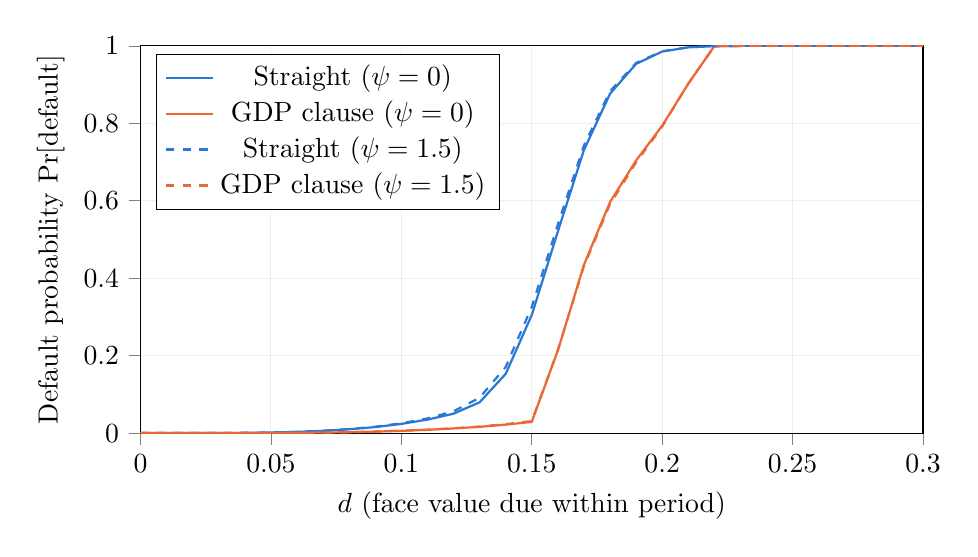
\begin{tikzpicture}
\begin{axis}[
  width=0.95\linewidth,
  height=6.5cm,
  xlabel={$d$ (face value due within period)},
  ylabel={Default probability $\Pr[\text{default}]$},
  legend style={at={(0.02,0.98)},anchor=north west},
  xmin=0, xmax=0.30, ymin=0, ymax=1,
  xtick={0,0.05,0.10,0.15,0.20,0.25,0.30},
  ytick={0,0.2,0.4,0.6,0.8,1},
  scaled x ticks=false, scaled y ticks=false,
  tick label style={/pgf/number format/fixed},
  x tick label style={/pgf/number format/fixed,/pgf/number format/precision=2},
  y tick label style={/pgf/number format/fixed,/pgf/number format/precision=1},
  grid=major, major grid style={opacity=0.25},
  tick align=outside, tick pos=left,
]
\addplot[vizblue, thick] coordinates {(0.00,0.0000) (0.01,0.0000) (0.02,0.0000) (0.03,0.0002) (0.04,0.0006) (0.05,0.0015) (0.06,0.0031) (0.07,0.0058) (0.08,0.0099) (0.09,0.0155) (0.10,0.0237) (0.11,0.0347) (0.12,0.0501) (0.13,0.0795) (0.14,0.1529) (0.15,0.3047) (0.16,0.5203) (0.17,0.7308) (0.18,0.8762) (0.19,0.9533) (0.20,0.9852) (0.21,0.9960) (0.22,0.9990) (0.23,0.9998) (0.24,0.9999) (0.25,1.0000) (0.26,1.0000) (0.27,1.0000) (0.28,1.0000) (0.29,1.0000) (0.30,1.0000)};
\addlegendentry{Straight ($\psi=0$)}
\addplot[vizorange, thick] coordinates {(0.00,0.0000) (0.01,0.0000) (0.02,0.0000) (0.03,0.0000) (0.04,0.0002) (0.05,0.0004) (0.06,0.0008) (0.07,0.0014) (0.08,0.0023) (0.09,0.0038) (0.10,0.0058) (0.11,0.0084) (0.12,0.0120) (0.13,0.0161) (0.14,0.0218) (0.15,0.0289) (0.16,0.2132) (0.17,0.4345) (0.18,0.5964) (0.19,0.7039) (0.20,0.7937) (0.21,0.9021) (0.22,0.9990) (0.23,0.9998) (0.24,0.9999) (0.25,1.0000) (0.26,1.0000) (0.27,1.0000) (0.28,1.0000) (0.29,1.0000) (0.30,1.0000)};
\addlegendentry{GDP clause ($\psi=0$)}
\addplot[vizblue, thick, dashed] coordinates {(0.00,0.0000) (0.01,0.0000) (0.02,0.0000) (0.03,0.0002) (0.04,0.0007) (0.05,0.0016) (0.06,0.0033) (0.07,0.0061) (0.08,0.0104) (0.09,0.0164) (0.10,0.0253) (0.11,0.0378) (0.12,0.0563) (0.13,0.0912) (0.14,0.1707) (0.15,0.3258) (0.16,0.5385) (0.17,0.7426) (0.18,0.8826) (0.19,0.9558) (0.20,0.9860) (0.21,0.9962) (0.22,0.9991) (0.23,0.9998) (0.24,0.9999) (0.25,1.0000) (0.26,1.0000) (0.27,1.0000) (0.28,1.0000) (0.29,1.0000) (0.30,1.0000)};
\addlegendentry{Straight ($\psi=1.5$)}
\addplot[vizorange, thick, dashed] coordinates {(0.00,0.0000) (0.01,0.0000) (0.02,0.0000) (0.03,0.0000) (0.04,0.0002) (0.05,0.0004) (0.06,0.0008) (0.07,0.0015) (0.08,0.0024) (0.09,0.0040) (0.10,0.0061) (0.11,0.0088) (0.12,0.0126) (0.13,0.0170) (0.14,0.0232) (0.15,0.0311) (0.16,0.2140) (0.17,0.4312) (0.18,0.5909) (0.19,0.6990) (0.20,0.7914) (0.21,0.9023) (0.22,0.9991) (0.23,0.9998) (0.24,0.9999) (0.25,1.0000) (0.26,1.0000) (0.27,1.0000) (0.28,1.0000) (0.29,1.0000) (0.30,1.0000)};
\addlegendentry{GDP clause ($\psi=1.5$)}
\end{axis}
\end{tikzpicture}
\caption{Default probability under straight vs.\ contingent debt (color distinguishes the contract; dashes the logistics scenario). The clause flattens the default transition in the intermediate-$d$ region by shifting repayments out of bad states; at $d=0.15$, default probability falls from 30\% to 3\%.}
\label{fig:pd}
\end{figure}

\subsection{Fiscal-limit gains and comparative statics}
\label{subsec:gains}

The policy-relevant question is not whether the curves shift but by how much, and under what conditions the gain is largest. Table~\ref{tab:msb_contracts} reports the maximizing face value $\widehat d^*$, peak proceeds $\widehat b^M$, the default probability at the maximizer, and the percentage gain in $\widehat b^M$ relative to straight debt, across clause types and logistics amplification.

\begin{table}[t]
\centering
\caption{Peak proceeds, default risk, and MSB gains across clause types and logistics amplification $\psi$. GDP clause: $\kappa=0.30$, $\bar g=0.95$; disaster clause: $\kappa_Z=0.35$. Monte Carlo, $N=200{,}000$; gains relative to straight debt at the same $\psi$.}
\label{tab:msb_contracts}
\begin{tabular}{@{}lccccc@{}}
\toprule
Contract & $\psi$ & $\widehat d^*$ & $\widehat b^M$ & $\widehat{PD}(\widehat d^*)$ & Gain vs.\ straight \\
\midrule
Straight & 0.00 & 0.135 & 0.11153 & 0.108 & --- \\
Straight & 0.75 & 0.134 & 0.11083 & 0.107 & --- \\
Straight & 1.50 & 0.133 & 0.10978 & 0.109 & --- \\
Straight & 2.25 & 0.133 & 0.10884 & 0.116 & --- \\
Straight & 3.00 & 0.133 & 0.10803 & 0.123 & --- \\
\addlinespace
GDP clause & 0.00 & 0.152 & 0.12320 & 0.030 & $+10.5\%$ \\
GDP clause & 0.75 & 0.152 & 0.12265 & 0.031 & $+10.7\%$ \\
GDP clause & 1.50 & 0.152 & 0.12208 & 0.033 & $+11.2\%$ \\
GDP clause & 2.25 & 0.152 & 0.12146 & 0.037 & $+11.6\%$ \\
GDP clause & 3.00 & 0.152 & 0.12084 & 0.041 & $+11.9\%$ \\
\addlinespace
Disaster clause & 0.00 & 0.136 & 0.11356 & 0.051 & $+1.8\%$ \\
Disaster clause & 0.75 & 0.136 & 0.11287 & 0.056 & $+1.8\%$ \\
Disaster clause & 1.50 & 0.136 & 0.11184 & 0.065 & $+1.9\%$ \\
Disaster clause & 2.25 & 0.135 & 0.11088 & 0.066 & $+1.9\%$ \\
Disaster clause & 3.00 & 0.135 & 0.11008 & 0.072 & $+1.9\%$ \\
\bottomrule
\end{tabular}
\end{table}

\begin{figure}[t]
\centering
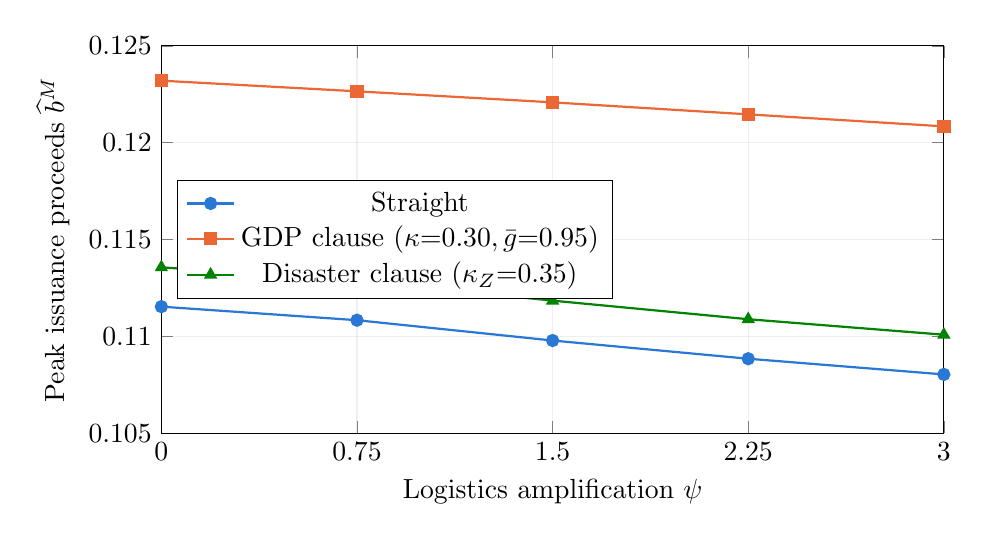
\begin{tikzpicture}
\begin{axis}[
  width=0.95\linewidth, height=6.5cm,
  xlabel={Logistics amplification $\psi$}, ylabel={Peak issuance proceeds $\widehat b^M$},
  xmin=0, xmax=3.0, ymin=0.105, ymax=0.125,
  xtick={0,0.75,1.5,2.25,3.0},
  scaled x ticks=false, scaled y ticks=false,
  tick label style={/pgf/number format/fixed},
  x tick label style={/pgf/number format/fixed,/pgf/number format/precision=2},
  y tick label style={/pgf/number format/fixed,/pgf/number format/precision=3},
  grid=major, major grid style={opacity=0.25},
  legend style={at={(0.02,0.5)},anchor=west},
]
\addplot[vizblue, thick, mark=*] coordinates {(0.00,0.11153) (0.75,0.11083) (1.50,0.10978) (2.25,0.10884) (3.00,0.10803)};
\addlegendentry{Straight}
\addplot[vizorange, thick, mark=square*] coordinates {(0.00,0.12320) (0.75,0.12265) (1.50,0.12208) (2.25,0.12146) (3.00,0.12084)};
\addlegendentry{GDP clause ($\kappa{=}0.30,\bar g{=}0.95$)}
\addplot[vizgreen, thick, mark=triangle*] coordinates {(0.00,0.11356) (0.75,0.11287) (1.50,0.11184) (2.25,0.11088) (3.00,0.11008)};
\addlegendentry{Disaster clause ($\kappa_Z{=}0.35$)}
\end{axis}
\end{tikzpicture}
\caption{Peak proceeds $\widehat b^M$ decline with logistics amplification $\psi$ under straight debt ($-3.1\%$ from $\psi=0$ to $\psi=3$), while the GDP clause both raises the level and flattens the decline ($-1.9\%$), so the contingency gain rises from $10.5\%$ to $11.9\%$ with centrality.}
\label{fig:msb_vs_psi}
\end{figure}

Four comparative statics answer the ``when is the gain largest?'' question.

\paragraph{(i) The gain grows with the rollover need.} Table~\ref{tab:gain_vs_d} fixes $\psi=1.5$ and compares proceeds contract-by-contract at given face values, rather than at the respective optima. At low rollover needs, the clause is a pure cost: at $d=0.08$, default is negligible under either contract, so the clause gives up payoff in survival states for no survival gain, and proceeds are 10\% \emph{lower}. The advantage turns positive just below the straight-debt peak and grows explosively beyond it: $+5\%$ at $d=0.14$, $+29\%$ at $d=0.15$, $+49\%$ at $d=0.16$. Contingent liabilities are valuable for sovereigns operating near their fiscal limits, not for sovereigns with ample headroom---which is also where the political demand for such instruments is found.

\begin{table}[t]
\centering
\caption{Proceeds advantage of the GDP clause by rollover need $d$ ($\psi=1.5$). The clause reduces proceeds when default risk is negligible and dominates near and beyond the straight-debt peak.}
\label{tab:gain_vs_d}
\begin{tabular}{@{}cccccc@{}}
\toprule
$d$ & $b_{\text{straight}}(d)$ & $b_{\text{GDP}}(d)$ & Advantage & $PD_{\text{straight}}$ & $PD_{\text{GDP}}$ \\
\midrule
0.08 & 0.0733 & 0.0658 & $-10.2\%$ & 0.010 & 0.002 \\
0.10 & 0.0903 & 0.0820 & $-9.1\%$ & 0.025 & 0.006 \\
0.12 & 0.1049 & 0.0980 & $-6.6\%$ & 0.056 & 0.013 \\
0.13 & 0.1094 & 0.1057 & $-3.3\%$ & 0.091 & 0.017 \\
0.14 & 0.1075 & 0.1133 & $+5.4\%$ & 0.171 & 0.023 \\
0.15 & 0.0936 & 0.1206 & $+28.8\%$ & 0.326 & 0.031 \\
0.16 & 0.0684 & 0.1020 & $+49.2\%$ & 0.539 & 0.214 \\
\bottomrule
\end{tabular}
\end{table}

\paragraph{(ii) The relative gain is invariant to surplus capacity $\alpha$.} This is an exact property, not a numerical finding:

\begin{remark}\label{rem:alpha_homog}
For any payoff mapping $H(g)$ that does not depend on $\alpha$, the problem \eqref{eq:default}--\eqref{eq:msbhat} is homogeneous of degree one in $(\alpha,d)$: replacing $\alpha$ by $c\alpha$ and substituting $d=c d'$ leaves the default event and price unchanged and scales proceeds by $c$. Hence $\widehat b^M(c\alpha)=c\,\widehat b^M(\alpha)$ for every contract, and percentage gains between contracts are independent of $\alpha$.
\end{remark}

Table~\ref{tab:gain_vs_alpha_mu} (top panel) confirms this numerically: as $\alpha$ ranges from 0.10 to 0.22, straight-debt capacity scales proportionally while the GDP-clause gain stays at $11.0\%\pm0.2$ percentage points (grid and Monte Carlo error) and the disaster-clause gain at $1.9\%$. The economic content is twofold. Low-$\alpha$ sovereigns benefit \emph{equally in proportional terms} but---precisely because their fiscal limits are lower---the same proportional gain relieves a binding constraint rather than adding unused headroom. And once $\alpha$ becomes stress-dependent as in \eqref{eq:alpha_endog}, the homogeneity breaks in favor of contingency: clauses deliver relief in exactly the states where $\alpha_t$ endogenously deteriorates. Quantifying that interaction requires the dynamic model and is left for future work.

\paragraph{(iii) The gain falls modestly as trend growth falls---with a fixed trigger.} The bottom panel of Table~\ref{tab:gain_vs_alpha_mu} varies mean log growth $\mu$ from $-0.02$ to $0.03$ per period. The GDP-clause gain \emph{declines} from 11.5\% to 10.3\% as $\mu$ falls, the opposite of the intuition that lower-growth countries benefit more. The reason is instructive: with the trigger fixed at $\bar g = 0.95$, a lower-growth country trips the clause in a larger share of \emph{non-default} states, so the payoff-reduction term in condition \eqref{eq:sufficient_condition} grows while the survival gain does not. The design lesson is that the trigger should be indexed to trend growth (e.g.\ $\bar g$ set relative to expected growth); with a trend-indexed trigger, the targeting of the clause---and hence the gain---is restored for low-growth issuers.

\begin{table}[t]
\centering
\caption{MSB gains from contingency as a function of surplus capacity $\alpha$ (top panel; $\mu=0.01$) and mean log growth $\mu$ (bottom panel; $\alpha=0.16$), at $\psi=1.5$. Gains are relative to straight debt in the same environment.}
\label{tab:gain_vs_alpha_mu}
\begin{tabular}{@{}ccccc@{}}
\toprule
 & $\widehat b^M_{\text{straight}}$ & Gain, GDP clause & Gain, disaster clause \\
\midrule
$\alpha=0.10$ & 0.0686 & $+11.2\%$ & $+1.9\%$ \\
$\alpha=0.13$ & 0.0892 & $+10.8\%$ & $+1.9\%$ \\
$\alpha=0.16$ & 0.1098 & $+11.2\%$ & $+1.9\%$ \\
$\alpha=0.19$ & 0.1304 & $+10.9\%$ & $+1.9\%$ \\
$\alpha=0.22$ & 0.1510 & $+11.2\%$ & $+1.9\%$ \\
\addlinespace
$\mu=-0.02$ & 0.1065 & $+10.3\%$ & $+1.9\%$ \\
$\mu=-0.01$ & 0.1076 & $+10.7\%$ & $+1.9\%$ \\
$\mu=0.00$ & 0.1087 & $+11.0\%$ & $+1.9\%$ \\
$\mu=0.01$ & 0.1098 & $+11.2\%$ & $+1.9\%$ \\
$\mu=0.02$ & 0.1109 & $+11.4\%$ & $+1.9\%$ \\
$\mu=0.03$ & 0.1120 & $+11.5\%$ & $+1.9\%$ \\
\bottomrule
\end{tabular}
\end{table}

\paragraph{(iv) The gain rises with tail thickness $\psi$.} From Table~\ref{tab:msb_contracts}: straight-debt capacity falls monotonically as logistics amplification thickens the left tail (from 0.1115 to 0.1080, $-3.1\%$), while GDP-clause capacity falls by only $-1.9\%$, so the contingency gain rises from 10.5\% to 11.9\%. This is the quantitative counterpart of Proposition~\ref{prop:psi_value} in Appendix~\ref{app:proofs}: a thicker left tail creates more probability mass that the clause can move from default to survival. Since $\psi$ proxies production-network centrality, the prediction is that high-centrality, import-dependent sovereigns gain the most from state contingency, holding local disaster risk constant.

The disaster clause's much smaller gain ($\approx 1.9\%$ throughout) is a quantified statement about \emph{basis risk}. The clause triggers on the observable event $Z=1$, but with exponentially distributed disaster sizes many triggered events are small (relief is wasted in survival states) while some untriggered states---deep Gaussian recessions, logistics-compounded downturns---still default (relief is missing where needed). The GDP clause conditions on the fiscally relevant object, output itself, and therefore dominates. In practice this trade-off runs the other way in verification costs: $Z$ is easier to verify than output shortfalls, which is why actual CRDCs use parametric triggers. The model quantifies what that verification convenience costs in fiscal space.

\subsection{Certain disasters: the $Z=1$ scenario}
\label{subsec:z1}

To make the ordering between GDP-linked bonds and disaster clauses fully explicit, Table~\ref{tab:z1} reports the degenerate scenario in which the disaster indicator is switched on with certainty ($Z=1$, jump drawn in every state; $\psi=0$).

\begin{table}[t]
\centering
\caption{The $Z=1$ scenario: disaster occurs with certainty. The disaster clause becomes a deterministic haircut---equivalent to rescaled straight debt---while the GDP clause retains its state contingency.}
\label{tab:z1}
\begin{tabular}{@{}lcccc@{}}
\toprule
Contract & $\widehat d^*$ & $\widehat b^M$ & $\widehat{PD}(\widehat d^*)$ & Gain vs.\ straight \\
\midrule
Straight & 0.106 & 0.07842 & 0.201 & --- \\
GDP clause ($\kappa{=}0.30,\bar g{=}0.95$) & 0.152 & 0.08839 & 0.204 & $+12.7\%$ \\
Disaster clause ($\kappa_Z{=}0.35$) & 0.163 & 0.07842 & 0.201 & $0.0\%$ \\
\bottomrule
\end{tabular}
\end{table}

The result is exact, not approximate: when the trigger is certain, $H_{\text{DIS}}=1-\kappa_Z$ in every state, so the disaster clause is a uniform haircut on face value---the sovereign simply issues $d/(1-\kappa_Z)$ units of a claim worth $(1-\kappa_Z)$ each, replicating straight debt state by state ($\widehat d^* = 0.106/0.65 \approx 0.163$, identical $\widehat b^M$ and default probability). The GDP clause, by contrast, still discriminates between the surviving and defaulting states \emph{within} the disaster environment and preserves a $+12.7\%$ gain. The ordering principle is that a contingent instrument creates fiscal space only insofar as its trigger is \emph{informative about the default set}; a trigger that fires always (or never) is payoff-equivalent to straight debt.

\subsection{Temperature-linked coupons and temperature-dependent disaster intensity}
\label{subsec:temp_sim}

This subsection carries the paper's two remaining announced extensions through the simulation: the temperature-linked instrument \eqref{eq:temp_linked} and the state-dependent jump intensity $\lambda(T_t)$ from \eqref{eq:jump_growth}.

Global emissions growth over the period is stochastic: $\Delta C/\overline{\Delta C}\sim$ lognormal with mean one and dispersion 0.30. It affects domestic growth through two couplings: the disaster intensity becomes $\lambda(\Delta C) = p_{\text{dis}} + \lambda_1(\Delta C/\overline{\Delta C}-1)$, so acute risk rises when global emissions overshoot; and a chronic wedge $\exp(-\delta_C(\Delta C/\overline{\Delta C}-1))$ scales growth directly. The temperature-linked coupon pays $H_T = 1-\kappa_T(\Delta C/\overline{\Delta C}-1)$: repayments fall when emissions overshoot (insurance) and rise symmetrically when they undershoot. Two coupling regimes are simulated: \emph{weak} ($\lambda_1=0.10$, $\delta_C=0.05$) and \emph{strong} ($\lambda_1=0.40$, $\delta_C=0.15$), at $\psi=1.5$.

\begin{table}[t]
\centering
\caption{Instrument comparison with stochastic global emissions and temperature-dependent disaster intensity $\lambda(\Delta C)$, at $\psi=1.5$. Weak coupling: $\lambda_1=0.10$, $\delta_C=0.05$; strong coupling: $\lambda_1=0.40$, $\delta_C=0.15$.}
\label{tab:temp}
\begin{tabular}{@{}lcccc@{}}
\toprule
Contract & $\widehat d^*$ & $\widehat b^M$ & $\widehat{PD}(\widehat d^*)$ & Gain vs.\ straight \\
\midrule
\multicolumn{5}{@{}l}{\emph{Panel A: weak coupling}} \\
Straight & 0.133 & 0.10955 & 0.110 & --- \\
GDP clause & 0.152 & 0.12197 & 0.033 & $+11.3\%$ \\
Disaster clause & 0.136 & 0.11164 & 0.066 & $+1.9\%$ \\
Temperature-linked ($\kappa_T{=}0.30$) & 0.129 & 0.10715 & 0.100 & $-2.2\%$ \\
\addlinespace
\multicolumn{5}{@{}l}{\emph{Panel B: strong coupling}} \\
Straight & 0.132 & 0.10752 & 0.120 & --- \\
GDP clause & 0.152 & 0.12127 & 0.039 & $+12.8\%$ \\
Disaster clause & 0.135 & 0.11060 & 0.068 & $+2.9\%$ \\
Temperature-linked ($\kappa_T{=}0.30$) & 0.131 & 0.10968 & 0.097 & $+2.0\%$ \\
Temperature-linked ($\kappa_T{=}0.50$) & 0.127 & 0.10672 & 0.089 & $-0.7\%$ \\
\bottomrule
\end{tabular}
\end{table}

Table~\ref{tab:temp} delivers a nuanced verdict on the paper's own proposed instrument, and reporting it honestly is the point of the exercise. Under weak coupling, the temperature-linked coupon \emph{reduces} the fiscal limit by 2.2\%: the global emissions realization is nearly orthogonal to the domestic default set at a five-year horizon, so the coupon adds payoff noise (and gives up repayments in overshoot states that are mostly survival states) without buying survival. Under strong coupling---when emissions overshoots substantially raise domestic disaster intensity and chronic damages---the same instrument turns positive ($+2.0\%$), comparable to the disaster clause; and overloading the coupon ($\kappa_T=0.50$) turns it negative again, the same interior-generosity logic as Section~\ref{subsec:kappa}. Two further observations: replacing the fixed intensity with the mean-preserving $\lambda(\Delta C)$ leaves straight-debt capacity essentially unchanged ($\widehat b^M$ moves by less than $10^{-4}$), so the value of the temperature link comes entirely from the \emph{correlation} it creates between the trigger and the default set, not from any change in average risk. And the one-period design understates the instrument's dynamic appeal: its natural role is to hedge the persistent BAU drift in cumulative emissions across periods---the state variable is global and trending---which a one-period exercise cannot capture. The practical-design comparison with catastrophe bonds and GDP-linked debt, including measurement and marketability concerns for small open economies, is taken up in Section~\ref{sec:conclusion}.

\subsection{Optimal clause generosity}
\label{subsec:kappa}

Condition \eqref{eq:sufficient_condition} predicts an interior optimum in relief generosity: increasing $\kappa$ raises the survival gain but also the payoff give-up in survival states. Figure~\ref{fig:msb_vs_kappa} varies $\kappa$ for the GDP clause at $\psi=1.5$ ($\bar g=0.95$). Peak proceeds rise from $\kappa=0.1$ to a maximum at $\kappa\approx 0.2$ ($\widehat b^M = 0.1237$), then decline monotonically---by $\kappa=0.8$ the clause is so generous that expected repayment collapses even though default is rare. The empirically relevant region for CRDC-scale deferrals ($\kappa\in[0.2,0.4]$) sits near the optimum, which is reassuring for practical design: contingency should be targeted and moderate, not maximal.

\begin{figure}[t]
\centering
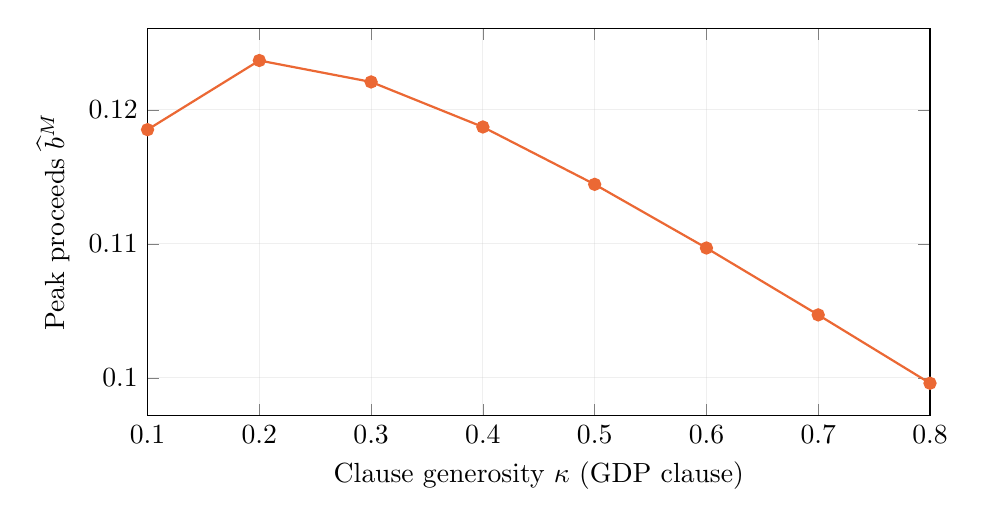
\begin{tikzpicture}
\begin{axis}[
  width=0.95\linewidth, height=6.5cm,
  xlabel={Clause generosity $\kappa$ (GDP clause)}, ylabel={Peak proceeds $\widehat b^M$},
  xmin=0.1, xmax=0.8,
  xtick={0.1,0.2,0.3,0.4,0.5,0.6,0.7,0.8},
  scaled x ticks=false, scaled y ticks=false,
  tick label style={/pgf/number format/fixed},
  x tick label style={/pgf/number format/fixed,/pgf/number format/precision=1},
  y tick label style={/pgf/number format/fixed,/pgf/number format/precision=3},
  grid=major, major grid style={opacity=0.25},
]
\addplot[vizorange, thick, mark=*] coordinates {(0.1,0.11852) (0.2,0.12368) (0.3,0.12208) (0.4,0.11872) (0.5,0.11444) (0.6,0.10969) (0.7,0.10470) (0.8,0.09960)};
\end{axis}
\end{tikzpicture}
\caption{Interior optimality in clause generosity. At $\psi=1.5$ and $\bar g=0.95$, proceeds peak at $\kappa\approx 0.2$: moderate relief maximizes the survival gain net of the payoff reduction in survival states, while overly generous relief destroys expected repayment even when default is rare.}
\label{fig:msb_vs_kappa}
\end{figure}

\section{Discussion and conclusion}
\label{sec:conclusion}

This paper started from an institutional fact---sovereigns such as Grenada and Barbados now write disaster contingency directly into their debt contracts---and asked what such design choices do to the maximum debt a government can sustain once climate risk is taken seriously. The answer, in a framework that extends the structural fiscal-limit tradition to acute physical risk and to a menu of contingent instruments, is that liability design is a quantitatively meaningful margin of climate policy. In the numerical illustration, a repayment clause that forgives about a third of payments in severe downturns raises the sustainable-borrowing benchmark by ten to twelve percent relative to conventional debt, while cutting the probability of default at the issuance optimum by roughly two-thirds. The gain is largest exactly where it matters: for sovereigns rolling over large amounts near their fiscal limit, for economies whose supply-chain position exposes them to disruptions originating elsewhere, and in environments where disasters make the distribution of growth outcomes more bottom-heavy. For sovereigns with ample headroom, the same clauses are a net cost---insurance bought against a risk they do not face.

Three design lessons emerge from the comparative statics. First, a contingent instrument creates fiscal space only insofar as its trigger tracks the states in which default would actually occur. A clause triggered by an event that is only loosely related to fiscal distress---our disaster clause with variable disaster sizes, or a temperature-linked coupon weakly coupled to domestic outcomes---delivers a small fraction of the gain, and in the limiting case of a trigger that always fires it delivers none at all, being equivalent to ordinary debt issued at a discount. This is the cost of verification convenience: parametric triggers are easy to verify but track fiscal distress imperfectly, and the model prices that basis risk at several percent of borrowing capacity. Second, relief should be moderate: the optimum forgives roughly a fifth to a third of payments in bad states, and more generous relief destroys value even when it makes default vanishingly rare. Third, triggers should be indexed to trend growth, since a fixed threshold becomes poorly targeted for slow-growing issuers.

The temperature-linked coupon deserves a candid practical assessment, since its trigger---global cumulative emissions---is measured with lags and model dependence, and no market for such instruments exists. Its comparative advantage over catastrophe bonds and GDP-linked debt is informational: a global emissions index cannot be manipulated by the issuing government (unlike output statistics, a known obstacle for GDP-linked bonds) and does not require loss verification after each event (unlike catastrophe triggers). Its disadvantages are that the trigger is outside any single issuer's control and, as the simulations show, only loosely coupled to a small economy's default states over short horizons. On this evidence, temperature-linked designs are best understood as long-horizon hedges of the global damage trend---complements to, not substitutes for, disaster clauses that handle acute local events. For small open economies, the credibility question is real but symmetric: precisely because the trigger is global, investors need not price moral hazard, but they must accept basis risk; which effect dominates is an empirical pricing question flagged for future work.

Several limitations bound these conclusions, and each defines a research direction. The quantitative exercise is a one-period illustration with a constant risk-free rate, not a calibrated welfare analysis: it prices instruments by risk-neutral investors, omits the continuation value of market access, and holds surplus capacity fixed even though the analytical framework allows capacity to deteriorate in stressed states---an extension under which the case for contingency would strengthen, since clauses deliver relief exactly when capacity erodes. The logistics-amplification channel is deliberately reduced-form; a full treatment would calibrate network centrality from input-output data and let disruption persist across periods, interacting with maturity choice. The monetary block in the appendix treats collateral policy and purchases analytically and through a simple comparative static, but does not solve the joint fixed point between pricing, default risk, and the risk-free rate that arises with long-maturity debt. And the framework's planner jointly chooses fiscal, debt-management, and monetary instruments---a useful benchmark, but one that abstracts from central bank independence; in practice, the coordination this paper studies would operate through institutionally separate mandates, with the central bank adjusting collateral treatment of instruments whose design independently reduces default risk, rather than through a single authority. Moral hazard and political economy also remain: relief is valuable precisely in bad states, so triggers must be verifiable and monitoring credible, and governments may prefer instruments that delay adjustment rather than hedge risk.

The empirical agenda is nonetheless sharp. The framework predicts that sovereign spreads respond less to qualifying disasters for issuers with credible disaster clauses; that this protection is worth more for trade-exposed, network-central economies; and that official-sector support---collateral eligibility, purchases---compresses premia most effectively when directed at instruments whose payoffs already reduce default risk. Each prediction is testable with event studies around disasters and shipping disruptions, spread regressions interacted with contractual features, and eligibility discontinuities.

The policy conclusion is continuous with the baseline literature but adds an operational margin. Coordinated mitigation remains the only durable answer to the long-run erosion of fiscal limits by climate damages. But while that coordination is negotiated, governments need not manage their balance sheets as if climate risk were not accumulating. Debt contracts that move repayments out of disaster states, priced transparently and triggered verifiably, buy fiscal room precisely when it is scarcest---and they do so through contract design, without inflation surprises, financial repression, or ex post renegotiation.

\section*{Code Availability}

All code associated with the simulations in this paper, including the revision simulations that generate every table and figure in Section~\ref{sec:numerical} and Appendix~\ref{app:monetary}, is available at: \url{https://osf.io/scugt}.

\printbibliography

\appendix

\section{Further relaxations of the baseline assumptions}
\label{app:further}

This appendix collects the relaxations of the baseline tractability assumptions that are analytically instructive but are not carried through the quantitative exercise of Section~\ref{sec:numerical}. They are presented as extensions of deliberate simplifications in \textcite{CollardEtAl2015} and \textcite{Seghini2026}, not as flaws in those frameworks.

\subsection{Maturity structure}
\label{app:maturity}

Assuming one-period debt fully rolled over each period makes MSB a static maximization of $d_t/R(d_t)$. But climate shocks are persistent and often arrive as clusters; maturity structure is therefore a first-order hedging margin (\cite{ChatterjeeEyigungor2012}; \cite{LorenzoniWerning2019}; \cite{BronerEtAl2013}). With long-term debt, the government can smooth rollover risk across states, and investors price a stream of contingent default probabilities. In a stylized $N$-period coupon bond, the gross promised return depends on the entire hazard path:
\begin{equation}\label{eq:long_debt_pricing}
P_t = \mathbb{E}_t\left[\sum_{k=1}^{N}\frac{\mathcal{C}_{t+k}\,\mathbb{1}\{\tau>t+k\}}{R_f^k}+\frac{\mathcal{F}\,\mathbb{1}\{\tau>t+N\}}{R_f^N}+\sum_{k=1}^{N}\frac{\mathcal{R}_{t+k}\,\mathbb{1}\{\tau=t+k\}}{R_f^k}\right],
\end{equation}
where $\mathcal{C}_{t+k}$ is the coupon paid at $t+k$, $\mathcal{F}$ is the face value repaid at maturity, $\tau$ is the default time, $\mathcal{R}_{t+k}$ is recovery in default, and $R_f$ is the gross risk-free rate.

The climate-specific reason maturity is first-order is that physical risks exhibit temporal clustering: extratropical cyclones and other hazard types arrive in serially correlated spells rather than independently across years (\cite{Mailier2006}), and reconstruction and repeated disruptions to ports, grids, and transport extend the macroeconomic footprint of each event. When rollover needs are concentrated at short horizons, clustered climate shocks mechanically push the sovereign into a sequence of refinancing states where spreads are highest, even if long-run fiscal capacity is unchanged. Conversely, terming out issuance before predictable increases in damages pre-commits the repayment schedule to states where market access is more reliable, flattening the endogenous default hazard embedded in \eqref{eq:long_debt_pricing}. Even if output growth were i.i.d., the default hazard is generally not, because debt stocks carry over; the one-period assumption thus tends to overstate the sensitivity of fiscal limits to near-term transition costs and understate the value of terming out issuance.

\subsection{Positive recovery}
\label{app:recovery}

Seghini assumes zero recovery, a standard simplification (\cite{CollardEtAl2015}). But recovery in advanced-economy restructurings is rarely zero, and the existence of official-sector facilities changes effective recovery values. With fractional recovery $\lambda\in(0,1)$, the pricing condition becomes
\begin{equation}\label{eq:pricing_recovery}
R(d_t)\Big( (1-\mathrm{PD}(d_t))+\lambda\,\mathrm{PD}(d_t)\Big)=R_f,
\end{equation}
so
\begin{equation}\label{eq:R_with_recovery}
R(d_t)=\frac{R_f}{1-(1-\lambda)\mathrm{PD}(d_t)}.
\end{equation}
Borrowing proceeds become
\begin{equation}\label{eq:proceeds_recovery}
b(d_t)=\frac{d_t}{R(d_t)}=d_t\frac{1-(1-\lambda)\mathrm{PD}(d_t)}{R_f}.
\end{equation}
Relative to zero recovery, positive recovery flattens $b(d)$ at high $d$ because default states no longer imply total investor losses. This mechanically raises MSB and MSD. Note that the baseline model, with its single instrument, contains no ranking of debt instruments; it is only once recovery (or contingency) varies across contract designs that such a ranking arises---e.g.\ clauses that increase recovery, such as maturity extensions with step-up coupons, can expand fiscal space without reducing ex ante borrowing proceeds.

\subsection{An endogenous risk-free rate}
\label{app:rf}

Fixing $R$ is conservative in some directions but not others. If physical damages raise global precautionary savings or trigger monetary easing, $R_f$ may fall, raising fiscal limits (Blanchard-type arithmetic). Conversely, climate risk can increase term premia and risk-free rates if it raises inflation volatility or risk aversion (\cite{Giglio2021}). For fiscal-limit analysis, what matters is that $R_f$ is itself a function of climate states and policy regimes:
\begin{equation}\label{eq:Rf_state}
R_{f,t}=R_f(\pi_t,\sigma_{\pi,t},\text{global risk},T_t),
\end{equation}
so that the borrowing factor is endogenous and potentially correlated with $g_{t+1}$. The simulations in Section~\ref{sec:numerical} hold $R_f$ constant; the fixed-point issues that arise once $R_f$ responds to purchases and default risk are discussed in Appendix~\ref{app:monetary}.

\subsection{State-dependent volatility}
\label{app:vol}

Seghini assumes the emissions path affects the mean of growth but not its volatility, which keeps the ``borrowing factor net of growth'' constant (\cite{Seghini2026}). Yet transition policy may increase short-run volatility (reallocation, energy-price shocks) and reduce long-run volatility (lower disaster exposure). Allowing $\sigma_t=\sigma(E_t,T_t)$ changes the maximizer $\gamma\equiv \max_x x[1-F(x)]$ because $F$ depends on $\sigma_t$. The MSB recursion becomes state-dependent:
\begin{equation}\label{eq:gamma_state}
b_t^M = \frac{\gamma(\sigma_t)\,e^{\mu_t}}{R_{f,t}}\big(\alpha_t+b_{t+1}^M\big)H_{t+1}.
\end{equation}
This is not a cosmetic change: if mitigation temporarily increases $\sigma_t$, the short-run fiscal-limit drop can be larger than the mean-growth channel suggests, even when the long-run benefits of lower $T_t$ dominate.

\subsection{Joint debt dynamics and endogenous adaptation}
\label{app:joint}

Seghini holds current debt ratios constant to isolate changes in fiscal limits (\cite{Seghini2026}). But policy design requires joint dynamics: debt may rise to fund adaptation, subsidies, and public investment (\cite{IMF2023FiscalMonitor}). Whether that is sustainability-enhancing depends on multipliers, the structure of liabilities, and the presence of state-contingent instruments. In principle the model can endogenize adaptation and public investment by letting $\mu_t$ or the disaster intensity $\lambda_t$ depend on an accumulated adaptation stock financed by issuance; the resulting problem couples the portfolio choice of Section~\ref{subsec:portfolio} to an investment Euler equation, and its calibration requires empirical multipliers for adaptation spending that are still scarce. This is a natural next step but beyond the present paper.

\section{Asset-market transmission: private equity and venture capital}
\label{app:pevc}

Sovereign climate risk transmits to private capital markets through both cash flows and discount rates; this appendix records the mapping used in the paper's discussion (it is not part of the quantitative exercise). Let a representative private equity or venture capital (PE/VC) asset in country $i$ have cash flows $CF_{i,t}$ exposed to climate and logistics shocks. Its value for global investors is
\begin{equation}\label{eq:asset_value}
V_{i,t} = \mathbb{E}_t\left[\sum_{s\ge 1} M^{\ast}_{t+s}\, CF_{i,t+s}\right],
\end{equation}
where $M^{\ast}$ is the global stochastic discount factor. Suppose cash flows scale with output and supply-chain reliability:
\begin{equation}\label{eq:cashflow}
\log CF_{i,t+1} = a + b\log Y_{i,t+1} - \nu \ell_{i,t+1} - \nu_T T_{t+1} + \eta_{i,t+1}.
\end{equation}
And suppose the global discount factor incorporates sovereign risk through financing conditions (exit discounting, local credit spreads, or required returns):
\begin{equation}\label{eq:SDF_with_sovereign}
M^{\ast}_{t+1} = \tilde M_{t+1}\exp\!\left(-\omega \pi_{i,t}\right),\quad \omega>0.
\end{equation}
Then sovereign climate risk reduces PE/VC values both by lowering expected cash flows and by raising discount rates (\cite{BoltonKacperczyk2021}; \cite{GiglioKellyStroebel2021}). This provides a welfare and political-economy rationale for instrument design: mitigating sovereign default risk protects the domestic tax base and stabilizes private capital values and cross-border investment. Once sovereign climate and logistics risk enters discounting \eqref{eq:SDF_with_sovereign} and cash flows \eqref{eq:cashflow}, the same shock that compresses fiscal space also mechanically reduces private-market valuations via a joint cash-flow and discount-rate channel---a concrete rationale for why global investors in illiquid assets should care about sovereign instrument design, especially in small open economies with large foreign investor bases.

\section{A monetary block: collateral policy, purchases, and inflation risk}
\label{app:monetary}

The fiscal-limit tradition on which this paper builds---\textcite{CollardEtAl2015}, extended by \textcite{CollardHabibPanizzaRochet2024}, and \textcite{Seghini2026}---deliberately excludes monetary finance. Yet climate policy is increasingly intertwined with central-bank operations: collateral frameworks, haircuts, refinancing terms, and portfolio tilts. This appendix incorporates monetary policy as a state-contingent liquidity backstop that affects sovereign pricing but is constrained by inflation risk and mandate credibility (\cite{IMF2023FiscalMonitor}). It is placed in an appendix because, as detailed below, its full equilibrium is not solved in this paper; a one-period comparative static on collateral haircuts is provided instead.

These channels have become operationally relevant. The Eurosystem has announced the introduction of a climate factor in its collateral framework, explicitly motivated by protecting the central bank balance sheet against climate-related transition risk and valuation uncertainty (\cite{ecb2025_climate_factor_pr}; \cite{ecb2025_climate_factor_faq}). In parallel, central banks (including the Bank of England) have expanded scenario analysis to assess climate-related financial risks in the asset classes most relevant to monetary operations, including sovereign bonds (\cite{boe2024_climate_scenario_analysis}; \cite{ngfs2025_scenario_guide_update}). These developments motivate modeling collateral haircuts and purchase eligibility as state-contingent policy levers rather than as neutral institutional background.

\subsection{Specification}

Let instrument $k$ be eligible collateral at haircut $h^k_t\in[0,1]$. Eligibility increases demand and lowers required returns. A reduced-form mapping for the premium is
\begin{equation}\label{eq:premium_haircut}
\pi^k_{i,t} = \pi_{i,t} - \xi (1-h^k_t),
\end{equation}
where $\xi>0$ is the effectiveness of collateral easing. Climate-tilted collateral policy can thus lower yields on resilience or temperature-linked instruments, increasing their issuance feasibility.

A natural instrument for such treatment is the \emph{resilience bond}, indexed to verified adaptation capital. Let $A_t$ denote the verified adaptation stock (flood defenses, grid hardening, wildfire prevention). A resilience bond's spread step-down can be represented by a lower payoff when adaptation progresses (because borrowing costs fall) or, equivalently, by an issuance price premium; a reduced-form payoff mapping is
\begin{equation}\label{eq:resilience_bond}
\Pi^5_{t+1}=1-\kappa_A \Delta A_t,
\end{equation}
where $\Delta A_t$ is verified progress and $\kappa_A>0$. This contract is implementable if monitoring and verification are credible, and it is the design for which prudential collateral treatment is easiest to justify: verified adaptation directly reduces the disaster exposure of the sovereign the central bank holds as counterparty.

Let the central bank purchase a share $\omega^k_t$ of instrument $k$. In segmented markets, purchases reduce term premia (\cite{KrishnamurthyVissingJorgensen2011}; \cite{GreenwoodVayanos2014}):
\begin{equation}\label{eq:term_premium}
\pi^k_{i,t} = \pi^k_{i,t}(\cdot) - \upsilon \omega^k_t.
\end{equation}
However, purchases are constrained by inflation and fiscal dominance risk. We \emph{assume}---this is a conjecture motivated by the fiscal-dominance arithmetic of \textcite{SargentWallace1981} rather than a derived result---that inflation variance $\sigma_{\pi,t}^2$ rises with large purchases of risky sovereign instruments:
\begin{equation}\label{eq:inflation_risk}
\sigma_{\pi,t}^2 = \bar\sigma_{\pi}^2 + \Gamma\sum_k \omega^k_t \mathrm{PD}(\bm{d}_t).
\end{equation}
The mechanism is that purchases of instruments with high default risk expose the central bank balance sheet to losses whose fiscal backing is uncertain, raising the variance of the future price level required to satisfy the consolidated budget constraint. Then $R_{f,t}$ may increase with $\sigma_{\pi,t}^2$ (risk/term premia), partially offsetting the direct benefit.

Consider a social planner (or coordinated authority) choosing emissions $\{E_t\}$, adaptation $\{A_t\}$, instrument shares $\{\bm{d}_t\}$, and monetary supports $\{\omega^k_t,h^k_t\}$ to maximize welfare:
\begin{equation}\label{eq:planner}
\max_{\{E_t,A_t,\bm{d}_t,\omega^k_t,h^k_t\}} \ \mathbb{E}_0\left[\sum_{t\ge 0}\beta^t U(C_t) - \Phi(\tau) - \Psi(\pi_t)\right]
\end{equation}
subject to: (i) the carbon budget \eqref{eq:carbon_budget}, (ii) temperature and damages \eqref{eq:damage}, (iii) growth dynamics with logistics \eqref{eq:growth_with_logistics}, (iv) fiscal feasibility \eqref{eq:default_multi}, and (v) monetary constraints linking $\omega,h$ to inflation risk \eqref{eq:inflation_risk}. Here $\Phi(\tau)$ is an expected default cost (output loss, financial instability), and $\Psi(\pi_t)$ is a penalty for inflation deviations. The single coordinated authority is a modeling benchmark: in advanced economies, central bank independence means the collateral and purchase decisions in \eqref{eq:premium_haircut}--\eqref{eq:term_premium} would be taken under a separate mandate, and the coordination studied here should be read as institutional consistency (the central bank recognizing the risk properties of well-designed instruments) rather than joint optimization.

\subsection{The pricing--default fixed point}

Equations \eqref{eq:premium}, \eqref{eq:premium_haircut}--\eqref{eq:inflation_risk} form a system in $(\pi,\mathrm{PD},R_f,\sigma_\pi)$: the premium is linear in PD, PD depends on pricing through $R(d)=R_f\exp(\pi)$ whenever repayment obligations are interest-bearing or multi-period, $\sigma_\pi$ depends on purchases of defaultable instruments, and $R_f$ feeds back through a term-premium channel. This paper does not solve that fixed point in general, and the simulations in Section~\ref{sec:numerical} hold $R_f$ constant. One special case is worth recording because it underlies the comparative static below: with one-period, zero-coupon debt and capacity $\alpha g$, the default event $dH(g)>\alpha g$ does not involve the issuance price, so $\mathrm{PD}(d)$ is determined before pricing and the system is \emph{recursive} rather than simultaneous---$\mathrm{PD}(d)$ first, then $\pi(d)=\theta_d \mathrm{PD}(d)-\xi(1-h)$, then proceeds. With long-maturity or interest-bearing debt the simultaneity is restored, and solving it is a prerequisite for any quantitative claim about monetary backstops; this is left to future work.

\subsection{A comparative static on collateral haircuts}

Within the recursive one-period case, the effect of collateral generosity on the fiscal limit can be computed exactly with the apparatus of Section~\ref{sec:numerical}. Let the eligible instrument be the GDP clause ($\kappa=0.30$, $\bar g=0.95$) at $\psi=1.5$, priced with premium $\pi(d)=\theta_d\,\mathrm{PD}(d)-\xi(1-h)$, $\theta_d=0.5$, $\xi=0.02$. Table~\ref{tab:haircut} sweeps the haircut $h$ from 1 (ineligible) to 0 (full collateral value).

\begin{table}[h]
\centering
\caption{Collateral haircut comparative static (GDP clause, $\psi=1.5$, $\theta_d=0.5$, $\xi=0.02$). Lower haircuts raise the fiscal limit through the pricing channel only; in the one-period model the default set---and hence $\widehat{PD}$ at the optimum---is unchanged.}
\label{tab:haircut}
\begin{tabular}{@{}ccccc@{}}
\toprule
Haircut $h$ & $\widehat d^*$ & $\widehat b^M$ & $\widehat{PD}(\widehat d^*)$ & Gain vs.\ ineligible \\
\midrule
1.00 & 0.152 & 0.12009 & 0.033 & --- \\
0.75 & 0.152 & 0.12069 & 0.033 & $+0.5\%$ \\
0.50 & 0.152 & 0.12130 & 0.033 & $+1.0\%$ \\
0.25 & 0.152 & 0.12191 & 0.033 & $+1.5\%$ \\
0.00 & 0.152 & 0.12252 & 0.033 & $+2.0\%$ \\
\bottomrule
\end{tabular}
\end{table}

Full eligibility raises the fiscal-limit analogue by about 2\%---roughly the size of the disaster clause's contractual gain---without changing the default set: in this setting collateral policy operates purely through the pricing channel. This sharpens the sense in which monetary support and instrument design are complements rather than substitutes: the haircut cannot substitute for a well-targeted trigger (it does not move repayments out of bad states), but it can amplify the issuance value of an instrument whose design has already reduced default risk.

Combining \eqref{eq:premium_haircut}--\eqref{eq:inflation_risk}, a sufficient condition for monetary support to increase MSB is
\begin{equation}\label{eq:monetary_condition}
\left|\frac{\partial \pi^k}{\partial \omega^k}\right| > \left|\frac{\partial \log R_{f,t}}{\partial \omega^k}\right|.
\end{equation}
The corresponding policy claim---that monetary backstops are most credible when conditioned on hedging instruments, because supporting instruments that lower PD limits the inflation-risk externality in \eqref{eq:inflation_risk}---should be read as a \emph{conjecture} supported by the comparative static above and by condition \eqref{eq:monetary_condition}, not as a theorem: proving it requires solving the fixed point with long-maturity debt and an operational inflation block.

\section{Proofs and formal results for the numerical experiments}
\label{app:proofs}

This appendix formalizes the results referenced in Section~\ref{sec:numerical}: (i) an interior optimum in clause generosity (Figure~\ref{fig:msb_vs_kappa}) and (ii) monotone comparative statics of clause value with left-tail thickening induced by logistics amplification $\psi$ (Figure~\ref{fig:msb_vs_psi}). The proofs build on the one-period fiscal-limit logic in \textcite{CollardEtAl2015} and its climate extension in \textcite{Seghini2026}, translated into the pricing/default representation in \eqref{eq:default}--\eqref{eq:iss_price}.

\subsection{Preliminaries and threshold structure}
Let $g>0$ be the next-period growth factor, $\alpha>0$ fiscal capacity, $R_f>1$ the gross risk-free rate,
and $H(g)\in(0,1]$ a measurable payoff mapping (possibly with parameters $\chi$ suppressed).
Define default as in \eqref{eq:default}: default occurs when $dH(g)>\alpha g$.

\begin{lemma}[Threshold structure of the default set]
\label{lem:threshold}
(i) Suppose $H(g)$ is weakly non-increasing in $g$; this covers straight debt, $H\equiv 1$, and countercyclical payoffs that \emph{raise} repayment in bad states. Then for every $d\ge 0$ there exists a threshold $g^*(d)$ such that the survival set is $\{g\ge g^*(d)\}$ (up to probability-zero sets), and the default probability is $PD(d)=\Pr(g<g^*(d))$.
(ii) The step-down clause $H_{\text{GDP}}(g)=1-\kappa\,\mathbf{1}\{g<\bar g\}$ with $\kappa\in(0,1)$ is instead weakly non-\emph{de}creasing, so it is not covered by (i); its survival set is
\[
\big[\,d(1-\kappa)/\alpha,\ \bar g\,\big)\ \cup\ \big[\,\max\{d/\alpha,\ \bar g\},\ \infty\,\big),
\]
which is an upper interval if and only if $d\le\alpha\bar g$ (in which case $g^*(d)=d(1-\kappa)/\alpha$) or $d\ge \alpha\bar g/(1-\kappa)$ (in which case $g^*(d)=d/\alpha$). On the intermediate range $d\in\big(\alpha\bar g,\ \alpha\bar g/(1-\kappa)\big)$ the default set is not a lower tail: states just above the trigger default while states just below it survive.
\end{lemma}

\begin{proof}
(i) Define $\phi_d(g)\equiv \alpha g - dH(g)$. Under the stated monotonicity, $\alpha g$ is increasing in $g$ and
$-dH(g)$ is weakly increasing in $g$, so $\phi_d(g)$ is increasing in $g$. Hence the survival set $\{g:\phi_d(g)\ge 0\}$ is an upper interval (possibly empty), i.e.\ $\{g\ge g^*(d)\}$ for $g^*(d)\equiv\inf\{g:\phi_d(g)\ge 0\}$. (ii) On $\{g<\bar g\}$ survival requires $d(1-\kappa)\le\alpha g$; on $\{g\ge\bar g\}$ it requires $d\le \alpha g$. Comparing the two induced cutoffs $d(1-\kappa)/\alpha$ and $d/\alpha$ with $\bar g$ yields the displayed set and the stated characterization.
\end{proof}

\begin{remark}\label{rem:threshold_window}
At the baseline calibration ($\alpha=0.16$, $\bar g=0.95$, $\kappa=0.30$) the non-threshold window in Lemma~\ref{lem:threshold}(ii) is $(\alpha\bar g,\ \alpha\bar g/(1-\kappa))=(0.152,\ 0.217)$. The proceeds maximizer of the GDP clause, $\widehat d^*=0.152=\alpha\bar g$ (Table~\ref{tab:msb_contracts}), sits exactly at the upper edge of the threshold branch, and the sharp rise of the clause's default probability over $d\in(0.152,\,0.217)$ in Figure~\ref{fig:pd} is the visible signature of the lost threshold structure. The results below use the threshold representation on the branch $d\le\alpha\bar g$, which contains the maximizer.
\end{remark}

Given Lemma~\ref{lem:threshold} (for the GDP clause, on the branch $d\le\alpha\bar g$; see Remark~\ref{rem:threshold_window}), the price and proceeds take the form
\begin{equation}
q(d)=\frac{1}{R_f}\, \mathbb{E}\!\left[H(g)\mathbf{1}\{g\ge g^*(d)\}\right], \qquad
b(d)=d\,q(d).
\label{eq:price_proceeds_app}
\end{equation}

\subsection{Interior optimality in clause generosity (formalizing Figure~\ref{fig:msb_vs_kappa})}

Consider the GDP-triggered clause $H_{\text{GDP}}(g;\kappa,\bar g)=1-\kappa\mathbf{1}\{g<\bar g\}$ with
$\kappa\in[0,1)$, and fix $\bar g$. Define peak proceeds $b^M(\kappa)=\max_{d\in\mathcal{D}} b(d;\kappa)$ for a compact grid $\mathcal{D}$.

\begin{proposition}[Interior optimal generosity under a survival--payoff trade-off]
\label{prop:interior_kappa}
Assume $g$ has a continuous density on $(0,\infty)$ and $\Pr(g<\bar g)>0$. Then there exist parameter regions in which $b^M(\kappa)$ is strictly quasi-concave in $\kappa$ on $[0,1)$ and attains an interior maximizer $\kappa^*\in(0,1)$.
\end{proposition}

\begin{proof}
Work on the threshold branch $d\le\alpha\bar g$ (Remark~\ref{rem:threshold_window}), where $g^*(d;\kappa)=d(1-\kappa)/\alpha$ and, with $F$ the CDF of $g$, proceeds are
\begin{equation}
b(d;\kappa)=\frac{d}{R_f}\Big[(1-\kappa)\big(F(\bar g)-F(g^*(d;\kappa))\big)+1-F(\bar g)\Big].
\label{eq:b_explicit_proof}
\end{equation}
Differentiating (with $f=F'$ the density) gives, for any fixed $d$,
\begin{equation}
\frac{\partial b(d;\kappa)}{\partial \kappa}
=
\underbrace{\frac{d}{R_f}\,(1-\kappa)\cdot \frac{\partial}{\partial \kappa}\Pr\!\left(g\ge g^*(d;\kappa)\right)}_{\text{survival gain, weighted by the marginal payoff }1-\kappa}
\;-\;
\underbrace{\frac{d}{R_f}\cdot \Pr\!\left(g<\bar g,\; g\ge g^*(d;\kappa)\right)}_{\text{payoff reduction in survival states}},
\label{eq:tradeoff_proof}
\end{equation}
where $\partial \Pr(g\ge g^*)/\partial\kappa=(d/\alpha)\,f(g^*(d;\kappa))$. The weight $1-\kappa$ appears because the marginal surviving states pay the clause payoff $1-\kappa$, not the full face value; at $\kappa=0$ the weight is unity and \eqref{eq:tradeoff_proof} reduces to the continuous analogue of \eqref{eq:sufficient_condition}. For small $\kappa$, the survival gain term can dominate because reducing repayments in low-$g$ states shifts $g^*(d;\kappa)$ downward and increases survival probability by an amount proportional to the density near the threshold. For large $\kappa$, survival probability saturates near one, the payoff reduction term increases toward $\Pr(g<\bar g)$, and the $1-\kappa$ weight attenuates the survival gain further, driving the derivative negative. Continuity and compactness of $\mathcal{D}$ imply the maximized objective $b^M(\kappa)$ inherits interior optimality under standard envelope/maximum theorem arguments.
\end{proof}

\subsection{Logistics amplification increases the value of properly targeted contingency (formalizing Figure~\ref{fig:msb_vs_psi})}

In the numerical model, logistics enters multiplicatively as $g=\exp(\mu+\varepsilon+J)\exp(-\psi L)$ with $L\ge 0$, so higher $\psi$ shifts probability mass toward low output states.

\begin{lemma}[First-order stochastic dominance shift]
\label{lem:fod_shift}
If $L\ge 0$ a.s.\ and independent of $(\varepsilon,J)$, then for $\psi_2>\psi_1$ the distribution of
$g(\psi_2)$ first-order stochastically dominates \emph{downward} $g(\psi_1)$:
$\Pr(g(\psi_2)\le t)\ge \Pr(g(\psi_1)\le t)$ for all $t>0$.
\end{lemma}

\begin{proof}
For any $t>0$, $\{g(\psi)\le t\} \Leftrightarrow \{\exp(\mu+\varepsilon+J)\le t\exp(\psi L)\}$.
Because $L\ge0$, increasing $\psi$ increases the right-hand side threshold in states with $L>0$, enlarging the event $\{g(\psi)\le t\}$ pointwise. Taking probabilities yields the result.
\end{proof}

\begin{proposition}[Comparative statics: clause value rises with tail thickening]
\label{prop:psi_value}
Let $b^M_{\text{GDP}}(\psi)$ and $b^M_{\text{straight}}(\psi)$ denote peak proceeds under the GDP clause
\eqref{eq:Hgdp} and straight debt \eqref{eq:Hstraight}. Suppose the clause is \emph{targeted} in the sense that
its trigger $\bar g$ lies in a neighborhood of the default threshold $g^*(d)$ for the straight-debt maximizer.
Then for sufficiently small but positive $\kappa$, the MSB gain
\[
\Delta b^M(\psi)\equiv b^M_{\text{GDP}}(\psi)-b^M_{\text{straight}}(\psi)
\]
is weakly increasing in $\psi$ over a neighborhood of the baseline, and strictly increasing when the density
near the threshold is positive and $\Pr(L>0)>0$.
\end{proposition}

\begin{proof}
By Lemma~\ref{lem:fod_shift}, increasing $\psi$ increases probability mass in the left tail.
Under straight debt, this increases the probability that $d>\alpha g$, reducing the survival term in
\eqref{eq:price_proceeds_app} at the maximizer. Under the GDP clause, repayment is reduced in the trigger region $g<\bar g$, which (by the targeting assumption) overlaps with the marginal default set created by the $\psi$-shift. Therefore the derivative of the survival gain term in \eqref{eq:tradeoff_proof} with respect to $\psi$ is positive at small $\kappa$ because a thicker left tail creates more mass that can be moved from default to survival by the clause. The payoff reduction term increases more slowly for small $\kappa$ because it is first-order in $\kappa$ but does not scale with the default boundary shift in the same way. Hence $\Delta b^M(\psi)$ rises locally in $\psi$, with strictness under positive mass in the logistics state $L>0$ and positive density near the threshold.
\end{proof}

\subsection{Consistency of the numerical MSB analogue}
Finally, the estimators \eqref{eq:qhat}--\eqref{eq:msbhat} converge to their population counterparts.

\begin{proposition}[Consistency of $\widehat b^M_N(\chi)$]
\label{prop:consistency}
Fix $\chi$ and assume $\mathbb{E}|H(g,\chi)|<\infty$.
Then $\widehat q_N(d;\chi)\to q(d;\chi)$ uniformly on a finite grid $\mathcal{D}$ a.s.\ as $N\to\infty$, and
$\widehat b^M_N(\chi)\to b^M(\chi)$ a.s.\ on $\mathcal{D}$.
\end{proposition}

\begin{proof}
For each fixed $d\in\mathcal{D}$, $\widehat q_N(d;\chi)$ is an average of integrable i.i.d.\ random variables, so it converges a.s.\ by the strong law of large numbers. Uniformity over a finite grid follows by a union bound over $\mathcal{D}$. The maximized value then converges because $\max_{d\in\mathcal{D}}$ is a continuous mapping on $\mathbb{R}^{|\mathcal{D}|}$.
\end{proof}

\end{document}
